

\chapter{Erwerbstätigkeit vs. Bildung - \newline
Die Wirkung des Freihandels auf die Humankapitalakkumulation eines Landes}
\chaptermark{Erwerbstätigkeit vs. Bildung}\label{Papier2}
\section{Intuition}

Humankapital und Sachkapital wird in Modellen häufig unter dem allgemeinen Begriff des Kapitals zusammengefasst.\footnote{Wie es beispielsweise im AK-Modell angenommen wird \cite{Rebelo.1991}.} Jedoch unterscheiden sich beide Kapitalarten deutlich hinsichtlich ihrer Wachstumswirkung, Herstellung und Abschreibung \cite{Ortigueira.1997}.\\
Dies zeigen auch Beispiele des letzten Jahrhunderts vor allem in Asien. In relativ kurzer Zeit wurden durch Investitionen in Kapital h{\"o}here Wachstumsraten erzielt worauf jedoch wirtschaftliche Krisen folgten. Der Grund f{\"u}r die zunehmenden Probleme lag unter anderem darin, dass zwar grunds{\"a}tzlich mehr Produktionsfaktoren in den Industriesektor investiert wurden, sich dadurch aber nicht die Produktivit{\"a}t erh{\"o}ht hat. Der Ausbau des Bildungssektors und die damit einhergehenden Investitionen in Humankaptial wurden  vernachl{\"a}ssigt, was den Mangel qualifizierter Arbeit und das Ausbleiben technologischer Neuerungen bedingte. Die effektivere Entwicklungsstrategie asiatischer L{\"a}nder k{\"o}nnte nun darin bestehen den gleichzeitigen Ausbau des Bildungssektors zu f{\"o}rdern und Technologien indirekt zu importieren, um drohenden Krisen entgegenzuwirken \citep{Krugman.2015}. \newline
Dieser indirekte Import birgt die Idee der globalen Wissensdiffusion durch Freihandel und der globalen Integration einer Volkswirtschaft. Beispielhaft für die Entwicklungsförderung durch den Wissenstransfer sind die ehemaligen Kolonien, die beispielsweise von kolonisatorisch implementierten Institutionen profitierten. Au{\ss}erdem konnte das technische Wissen sowie Fähigkeiten der Kolonialmächte übernommen werden. Dieser Humankapitaltransfer führte dazu, dass einige Volkswirtschaften wie Ägypten oder Südafrika heute weiter entwickelt sind als direkte Nachbarn mit ähnlichen Ausgangsbedingungen wie Libyen oder Mosambik \citep{Acemoglu.2000b}.\\
Auch das Beispiel der Pharmaindustrie soll die Möglichkeiten internationalen Wissenstransfers verdeutlichen. Werden in relativ weit entwickelten Ländern Medikamente, wie beispielsweise Impfstoffe durch vorwiegend gentechnische Verfahren in Bakterienkulturen hergestellt, deren Produktion somit sehr humankapitalintensiv ist, so ist der Prozess in weniger weit entwickelten Ländern zur Produktion dieser Impfstoffe noch durch traditionelle Verfahren geprägt.\footnote{Hier werden biochemische Prozesse im Labor nicht künstlich hervorgerufen, sondern Resistenzen direkt bei vorher infizierten Tieren gewonnen. Die anschlie{\ss}end isolierten Antikörpern können auf den Menschen übertragen werden \citep{Aberle.2010}.} Dieses Beispiel zeigt unterschiedliche Verfahrensmöglichkeiten verschiedener Entwicklungsstadien von Volkswirtschaften auf, und, dass ein Import des Impfstoffes einerseits die Ressourcen des Landes langfristig schonen würde sowie direkt zu einem Wissenstransfer führt, der eine mögliche Imitation des Gutes grundsätzlich nicht ausschlie{\ss}t. Unabhängig von dem Import der Güter ist für die Imitation die Qualifikation und somit die Bildung der Bevölkerung notwendig, um diesen Wissenstransfer umfassend ausnutzen zu können. \\
Diesem kausalen Zusammenhang folgend, soll gezeigt werden, dass sich ein Land durch den Import von Humankapital besser stellt,  ohne dabei jedoch Migration in die Modellwelt zu integrieren. Koppelt man den Ideenfluss zwischen zwei L{\"a}ndern, der auch als Wissensfluss interpretiert werden kann, an den G{\"u}terfluss, dann wird indirekt Humankapital importiert \citep{RiveraBatiz.1991a}.\\
Der Kerngedanke ist, dass das Wachstum eines weniger weit entwickelten Landes ansteigt, wenn Güter importiert werden, die mit relativ viel Humankapital produziert wurden. Es folgt ein langfristiger Effekt bezüglich der Ressourcen durch Faktormehrung im Bildungssektor. Denn je mehr von diesem Gut importiert wird, desto weniger muss davon im Land selbst produziert werden und es kann dadurch die Produktionsfaktoren umverteilen. In der folgenden Modellwelt bedeutet dies, dass nun das eingesparte Humankapital die Humankapitalakkumulation fördert. Jedoch führt ein Import von humankapitalintensiv produzierten Gütern auch zu einem kurzfristigen Effekt des einmaligen Wissenstransfers. Mit dem Gut wird ebenso technisches Wissen transferiert und führt zu einem Erkenntnisgewinn. Technologien, Verfahren und Einsatzfaktoren können analysiert werden, um diese zu einem späteren Zeitpunkt zu imitieren.\footnote{Die Imitation der Güter führt dann wiederum zu einem langfristigen Effekt dieses Imports auf die Wachstumsrate, jedoch wird in dieser Modellwelt nicht zwischen innovierenden und imitierenden Fähigkeiten unterschieden und lediglich auf das Bildungsniveau hingewiesen. Zwar geht mit einem höheren Bildungsniveau auch eine höhere Wahrscheinlichkeit einher innovieren zu können, wird jedoch an dieser Stelle vorerst vernachlässigt und nicht modelliert.}
Neben diesen beiden Effekten steigt mit der Einfuhr von Gütern auch die Nachfrage nach Humankapital, um langfristig eine Adaption anzustreben, kurzfristig jedoch um die Güter gezielt einzusetzten und sachgerecht anwenden zu können. Demzufolge liefert Handel den Anreiz Qualifikationen auszubauen. \\
Das endogene Wachstumsmodell von \citet{RiveraBatiz.1991a} bildet einen Forschungssektor ab, der nur mit dem Einsatz von Humankapital arbeitet. Sie untersuchen ebenfalls die Effekte internationaler Integration auf das Wachstum und zeigten, dass Handel keinen Einfluss auf das Wachstum des Weltmarktes hat, sofern der Forschungssektor nur Humankapital als Ressource einsetzt \citep{RiveraBatiz.1991a}. \citet{Devereux.1994} f{\"u}hren diesen Gedanken fort und {\"u}berpr{\"u}fen erneut die These \citep{RiveraBatiz.1991a}. Dabei stellen sie fest, dass sie lediglich dann stimmt, wenn es sich hinsichtlich der Humankapitalausstattung im Autarkiezustand um exakt gleiche L{\"a}nder handelt. Sobald es auch nur einen geringen Unterschied in der Ausstattung gibt, spezialisiert sich im Zuge der Integration das Land mit der h{\"o}heren Humankapitalausstattung auf den Forschungsbereich \citep{Devereux.1994}. Daraus lässt sich für dieses Modell ableiten, dass das relativ weiter entwickelte Land ein Gut exportieren, das relativ humankapitalreich ist.\footnote{Diese Handelsstruktur ergibt sich nach dem Heckscher-Ohlin-Theorem.} Somit wird der Faktor Humankapital, das technische Wissen, indirekt exportiert und mindert dadurch den möglichen Einsatz im heimische Bildungssektor. Dies legt die Vermutung nahe, dass die Humankapitalakkumulation zurück geht. Hinzu kommt, dass durch den beschriebenen Wissenstransfer der Export den Wissensvorsprung gegenüber den weniger weit entwickelten Ländern mindert. Dies hat wirtschaftliche Konsequenzen und demzufolge auch einschränkende Wirkung auf das Wachstum der Volkswirtschaft. Die folgende Imitation des Gutes in anderen Ländern führt weltweit zu Substituten und mindert dadurch die Marktmacht und den Preissetzungsspielraum. Freihandel steigert somit den Wettbewerb. Langfristig führt dies jedoch dazu, dass eine Kontinuität der Innovationsentwicklung in relativ weiter entwickelten Ländern herrschen muss um anhaltendes Wachstum aufrecht zu erhalten. \\
Das folgende endogene Wachstumsmodell legt den Schwerpunkt auf den Bildungssektor und  beschränkt sich zunächst lediglich auf die langfristige Wirkung bezüglich der Faktorumverteilung durch Au{\ss}enhandel und den einmaligen Wissenstransfer. Dabei soll eine Verzögerung des Entwicklungsprozesses durch den technologischen Fortschritt aufgrund eines Mangels an qualifizierten Arbeitskräften verhindert werden.\\
In dem später folgenden Modell in Kapitel \ref{Papier1} ist qualifizierte Arbeit notwendig, um imitierend oder innovierende Tätigkeiten auszuüben. Diese langfristigen Folgen werden hier noch ausgeblendet und erst zu einem späteren Zeitpunkt wieder aufgegriffen. \\


\section[Das Uzawa-Lucas-Modell]{Das Uzawa-Lucas-Modell\sectionmark{Uzawa-Lucas-Modell}}
\sectionmark{Uzawa-Lucas-Modell}
Das Uzawa-Lucas-Modell beschreibt das Wachstum einer Volkswirtschaft durch die Humankapitalakkumulation und vermittelt dabei die Bedeutung des Bildungssektors f{\"u}r die Entwicklung eines Landes. In dieser reduzierten Modellwelt geht ein erh{\"o}htes Wachstum des Humankapitals mit daraus resultierendem Wirtschaftswachstum einher. Denn der Zuwachs fundamentaler F{\"a}higkeiten wie beispielsweise die Alphabetisierung führt zu einem Anstieg der Produktivit{\"a}t des einzelnen und letztlich der gesamten Volkswirtschaft \citep{Romer.1990}. Demnach ist ein dauerhaftes Wachstum des Pro-Kopf-Einkommens m{\"o}glich, sofern beide Kapitalst{\"o}cke gleichm{\"a}{\ss}ig aufgebaut werden, weil die partiellen Grenzprodukte des Sach- und Humankapitals nicht abnehmen.\newline Dieses Modell dient als Grundlage und Ausgangssituation f{\"u}r die folgenden Modellvariationen von offenen Volkswirtschaften, in denen der Bildungssektor eine vorherrschende Rolle spielen wird.
Die Lebenszeit der Haushalte ist nicht begrenzt und somit kommt es zu keinem Wissensverlust. Sie k{\"o}nnen sich entscheiden, wie sie ihre Kapazit{\"a}ten auf die beiden Sektoren Bildung und Produktion aufteilen. Ihnen stehen nur diese zwei Alternativen zur Verf{\"u}gung. Somit haben sie die Wahl zwischen der Arbeit in einem Produktionsbetrieb, um Einkommen f{\"u}r ihren Lebensunterhalt zu verdienen, oder aber den Ausbau und der Vertiefung ihrer Qualifikationen im Bildungssektor, um ihre zuk{\"u}nftige Produktivit{\"a}t zu steigern.
Das Uzawa-Lucas-Modell geht insgesamt von $L$ Arbeitern aus mit F{\"a}higkeiten in H{\"o}he von $h(t)$, mit $0 \le h(t)\leq \infty$.\newline Die F{\"a}higkeiten $h(t)$ eines Arbeiters werden auch als Humankapital bezeichnet. Die H{\"o}he des Humankapitalbestandes wirkt sich in zweierlei Hinsicht positiv auf die Volkswirtschaft aus. Es gibt einen internen Effekt, dabei steigert ein h{\"o}herer Humankapitalbestand die Produktivit{\"a}t eines Arbeiters und einen externen Effekt, bei dem der durchschnittliche Humankapitalbestand einer Gesellschaft $h_a$ steigt, wenn sich die Qualifikation eines einzelnen verbessert. \newline Der Effekt wird als extern bezeichnet, weil alle Teilnehmer einer Gesellschaft von dem Zuwachs an Humankapital profitieren k{\"o}nnen und keine einzelne individuelle Entscheidung direkten Einfluss auf $h_a$ hat. Somit geht Humankapitalakkumulation mit positiven Externalitäten einher. Dieser Einfluss wird bei der individuellen Entscheidung {\"u}ber die Zeit nicht ber{\"u}cksichtigt und ist somit exogen. \newline Wird davon ausgegangen, dass alle Arbeiter $L$ gleich sind und auch mit den gleichen F{\"a}higkeiten, also Humankapital ausgestattet sind, dann wird die Bev{\"o}lkerung beschrieben als $N=u(t)h(t)L$, wobei gilt, dass $h_a(t)=h(t)$ ist.\newline Die Technologie f{\"u}r die G{\"u}terproduktion wird formal folgenderma{\ss}en ausgedr{\"u}ckt:
\begin{equation}
N(t)c(t)+\dot{K}(t)=AK(t)^\beta[u(t)h(t)N(t)]^{1-\beta}h_a(t)^\gamma \label{TechnologieLucas}
\end{equation} 
Die Produktionsfunktion zeigt den Einfluss der verschiedenen Parameter auf den Herstellungsprozess. Bei $h(t)$ handelt es sich um den Humankapitalbestand eines repr{\"a}sentativen Haushalts. Der Anteil der Kapazit{\"a}t eines Arbeiters, den er f{\"u}r die Herstellung von G{\"u}tern aufwendet, wird mit $u(t)$ bezeichnet. Der externe Effekt des Humankapitals wird durch $h_a(t)$ dargestellt und $A$ beschreibt das konstante Technologielevel der Volkswirtschaft.\footnote{Bei den übrigen Variablen handelt es sich um die gewohnten Bezeichnungen. $c(t)$ steht für die konsumierte Menge der Gütereinheiten. $K(t)$ steht für das physische Kapital, in diesem Fall der Veränderung des Kapitals über die Zeit, $\dot{K}(t)$. $\beta$ und $\gamma$ sind die jeweiligen Produktionselastizitäten.} \newline Die Akkumulation des Humankapitals folgt der Idee von \citet{Uzawa.1965}.
\begin{equation} 
\dot{h}(t)=h(t)\delta(1-u(t)) 
\end{equation} 
Diese Gleichung zeigt die Bildung des Humankapitals abhängig von der Entscheidung des Individuums. So hat es die Wahl zwischen der Güterproduktion mit einem Anteil von $u(t)$ oder der Weiter- und Ausbildung mit einem Anteil von $(1-u(t))$. \citet[Kapitel 13]{Aghion.2015} beschrieben diesen Term auch als den Einfluss des aktuellen Bildungsaufwands auf die Humankapitalakkumulation. Die Wachstumsrate des Humankapitals $h(t)$ wird mit $\delta$ bezeichnet \citep[S.~17--19]{Lucas.1988}.
Die Annahme konstanter Skalenertr{\"a}ge der Humankapitalakkumulation bez{\"u}glich des Humankapitalbestandes f{\"u}hrt zu konstanten Wachstumsraten im Steady-state.\\
Nach Vernachlässigung der Abhängigkeit zu der Zeit $t$ lässt sich die Bewegungsgleichung $\dot{K}$ aus der Umformulierung von Gleichung \eqref{TechnologieLucas} herleiten.
\begin{equation}
\dot{K}=AK^\alpha(uhN)^{1-\beta}-Nc
\end{equation}
Sie beschreibt die Ver{\"a}nderung {\"u}ber die Zeit des Sachkapitals bzw. physischen Kapitals. Der Kapitalstock bildet sich aus dem realisierenden Einkommen abz{\"u}glich des Konsums \citep{Aghion.2015}.\footnote{Ebenso verhält es sich im Solow- oder Ramsey-Modell.}
Das Modell wird unter zu Hilfenahme der Hamiltonfunktion optimiert. 
\begin{equation}
\mathbb{H}=\frac{N}{1-\sigma}(c^{1-\sigma}-1)+\lambda_1[AK^\beta(uNh)^{1-\beta}h^\gamma-Nc]+\lambda_2[\delta h(1-u)]
\end{equation}
Der Lebenszeitnutzen, definiert {\"u}ber die Nutzenfunktion $\frac{N}{1-\sigma}(c^{1-\sigma}-1)$, wird maximiert unter Ber{\"u}cksichtigung beider Kapitalrestriktionen. \newline Ein Individuum steht in diesem Modell zwei Entscheidungen gegen{\"u}ber, bez{\"u}glich des Konsums und der Humankapitalaufteilung, folglich gibt es auch zwei Entscheidungsvariablen, $c$ und $u$, sowie die beiden Zustandsvariablen $k$ und $h$. \newline Das Gut muss demnach in zweierlei Hinsicht gleichwertig sein, bzw. in diesen Bereichen gleich wichtig sein. Zum einen durch den reinen Konsum an sich und zum anderen in der Kapitalakkumulation. Der Schattenpreis erm{\"o}glicht es den Nutzenzuwachs intertemporal mit einander zu vergleichen. Der direkte Konsum liefert Nutzen, wohingegen die zuk{\"u}nftige Sachkapitalakkumulation einen monet{\"a}ren Mehrwert liefert, der sich erst durch den Schattenpreis als Nutzen interpretieren l{\"a}sst.  Diesen Zusammenhang beschreibt die Bedingung erster Ordnung, $\frac{\partial H}{\partial k}=-\dot{\lambda}_1$. Sie sagt aus, dass im Gleichgewicht ein Anstieg des Kapitalstocks mit der Ver{\"a}nderung des Schattenpreises {\"u}bereinstimmen muss. \newline 
Auch der Anteil $u$ muss sowohl in der Humankapitalakkumulation, als auch in der Produktion von G{\"u}tern gleich viel wert sein. Dies wird durch die optimale H{\"o}he der Aufteilung des Humankapitals bedingt aus $\frac{\partial H}{\partial u}=0$, die bei einer {\"U}bereinstimmung der Humankapitalver{\"a}nderung mit dem Schattenpreis des Humankapitals den gr{\"o}{\ss}t m{\"o}glichen Nutzen stiftet, bedingt durch $\frac{\partial H}{\partial h}=-\dot{\lambda}_2$ \cite[S.~20--21]{Lucas.1988}.\\
Auf die detaillierte  Berechnungen des Uzawa-Lucas-Modells wird in dieser Arbeit verzichtet und nur der gleichgewichtige konstante Konsumpfad gem{\"a}{\ss} der Keynes-Ramsey-Regel vorgestellt.
\begin{equation}
\hat{c}(t)=\frac{1}{\sigma}(\delta-\rho)
\end{equation}
In ihrer {\"u}blichen Form beschreibt sie das Konsumwachstum bedingt durch die Zeitpr{\"a}ferenzrate $\rho$ und die Wachstumsrate des Humankapitlas $\delta$. Je h{\"o}her die Pr{\"a}ferenz eines Individuums f{\"u}r den heutigen Konsum ist, also je gr{\"o}{\ss}er die Zeitpr{\"a}ferenzrate, desto weniger kann in der Zukunft konsumiert werden, desto kleiner ist demnach die Wachstumsrate. Hinsichtlich des Wachstums des Humankapitals l{\"a}sst sich sagen, dass mit einer steigenden Wachstumsrate auch das Konsumwachstum $\hat{c}$ ansteigt. Solange dieses die H{\"o}he der Zeitpr{\"a}ferenzrate {\"u}bersteigt, wird ein positives Wirtschaftswachstum resultieren.\bigskip

Der folgende Abschnitt wird auf die Unterschiede der beiden urspr{\"u}nglichen Ans{\"a}tze von \citet{Uzawa.1965} bzw. \citet{Lucas.1988} eingehen und zeigen, warum eine Modifikation des Modells nach \citet{Uzawa.1965} notwendig war. Anschlie{\ss}end werden einige Modellvariationen angeführt, die die Vielfalt des Aussagegehalts des Modells wiederspiegeln sollen.\\
\citet{Uzawa.1965} zeigt in seinem Modell ein Wachstum des Pro-Kopf-Einkommens, das nur durch die endogene Entwicklung des Humankapitalbestandes bedingt wird, \citet{Lucas.1988} hingegen erweitert dieses Modell um einen externen Wachstumsanreiz, indem positive Externalitäten in Form von Wissensdiffusion angenommen wird.\newline Ein weiterer Unterschied beider Ans{\"a}tze liegt darin, dass \citet{Lucas.1988} einzelwirtschaftlich von abnehmenden Ertr{\"a}gen der Humankapitalakkumulation ausgeht, wohingegen \citet{Uzawa.1965} eine Linearit{\"a}t derselben annimmt. Zu Beginn eines Lebens ist die Priorit{\"a}t Humankapital zu akkumulieren recht hoch, sinkt jedoch mit dem Alter. Jede neu hinzuerworbene F{\"a}higkeit muss aufwändiger verdient bzw. erworben werden. So ist es beispielsweise mit zunehmendem Alter m{\"u}hsamer Sprachen zu lernen als in jungen Jahren. \cite{Lucas.1988} best{\"a}tigt zwar, dass auch abnehmende Ertr{\"a}ge in der Realit{\"a}t beobachtet werden und diese in seinem Ansatz ber{\"u}cksichtigt wurden, jedoch nicht vornehmlich zum Ergebnis beitragen. Dieses Argument wird durch verschiedene Perspektiven gelöst. Optimiert ein Haushalt seinen Lebenszeitnutzen, dann berücksichtigt er bei seinen Entscheidungen nicht zwingend alle gesamtwirtschaftlichen Externalitäten. Schaut jedoch der soziale Planer auf das Optimierungsproblem, werden jegliche Zusammenhänge berücksichtigt. Hinzu kommt, dass \citet{Uzawa.1965} nicht den durchschnittlichen Humankapitalbestand einer Gesellschaft betrachtet und somit externe Effekte vernachl{\"a}ssigt, so dass gesamtwirtschaftlich keine abnehmenden Grenzerträge resultieren. \citeauthor{Uzawa.1965}s \citeyear{Uzawa.1965} Ansatz sei demnach eine Sackgasse, weil kein dauerhaftes Wachstum folgen w{\"u}rde \cite[S.~19]{Lucas.1988}.\\
Laut \citet{Lucas.1988} bleiben die Bildungsertr{\"a}ge konstant und ver{\"a}ndern sich auch nach dem Tod eines Individuums nicht. Diesen Kritikpunkt greifen \cite{Azariades.1990} in einem OLG-Modell auf und modellieren die {\"U}bertragung des vorhandenen Wissens auf folgende Generationen. Diese Vererbung von Humankapital f{\"u}hrt jetzt jedoch zu multiplen Steady States und somit zu keiner eindeutigen Lösung.\footnote{Sie zeigen au{\ss}erdem in ihrer Modellabwandlung, dass verschieden ausgestattete L{\"a}nder, mit unterschiedlichem Humankapitalbestand, nicht zwingend konvergieren, sondern mit verschiedenen Raten wachsen k{\"o}nnen.}\newline 
\citet{SalaiMartin.1996} best{\"a}tigen die Ergebnisse \citeauthor{Lucas.1988}' \citeyear{Lucas.1988} empirisch und zeigen, dass in den Jahren zwischen 1965 und 1985 ein positiver Effekt der Bildung auf das Wachstum ausging.\\
Eine weitere Abwandlung des Uzawa-Lucas-Modells wurde von \citet{Ortigueira.1997} vorgestellt. Ihr endogenes Wachstumsmodell ber{\"u}cksichtigt neben der Humankapitalakkumulation auch die Akkumulation des physischen Kapitals. Sie untersuchen die Konvergenzgeschwindigkeit zum gleichgewichtigen Wachstumspfad. Dabei stellen sie fest, dass die Wachstumsrate in erster Linie von den technischen Parametern abh{\"a}ngt. Au{\ss}erdem kommen sie zu dem Ergebnis, dass die Konvergenzgeschwindigkeit mit der Humankapitalproduktivit{\"a}t steigt und mit dem Ertrag des Sachkapitals im Konsumgutsektor sinkt. Dies verdeutlicht, warum es sinnvoll sein kann, das Humankapital vom physischen Kapital in einer Modellformulierung zu differenzieren \citep{Ortigueira.1997}.\\
\newline
Im ursprünglichen Uzawa-Lucas-Modell ist das physische Kapital im Humankapitalsektor nicht produktiv. Daraus ergibt sich auch, dass es keine Aufteilung des Sachkapitals auf den Bildungssektor und den Produktionssektor gibt.\newline Diese Situation ist denkbar in relativ weniger weit entwickelten L{\"a}ndern, die das absolut knappe physische Kapital vollst{\"a}ndig f{\"u}r die G{\"u}terproduktion verwenden. Der Bildungssektor wird nur durch den Einsatz von Humankapital aufrecht erhalten, das absolut gesehen im Vergleich mit industrialisierten L{\"a}nder ebenfalls knapp ist. Relativ gesehen wird ein weniger weit entwickeltes Land jedoch tendenziell {\"u}ber mehr physisches Kapital verf{\"u}gen als {\"u}ber Humankapital. \newline In dem folgenden Kapitel \ref{Papier2} wird neben dem gerade beschriebenen Fall weniger weit entwickelter Volkswirtschaften auch ein Bildungssystem berücksichtigt, in dem neben Humankapital auch das physische Kapital eingesetzt wird. Denn in relativ weiter entwickelten Volkswirtschaften stehen beide Produktionsfaktoren ausreichend zur Verf{\"u}gung und können in beiden Sektoren produktiv eingesetzt werden.
%Sofern ein gleichmä{\ss}iger Aufbau der Kapitalstöcke stattfindet, nehmen die partiellen GP nicht ab und ein dauerhaftes Wachstum des Pro-Kopf-Einkommens ist möglich. (V-Soretz)


\section[Vorstellung der Modellvariationen]{Vorstellung der Modellvariationen\sectionmark{Modellvariationen}}
\sectionmark{Modellvariationen}
Die Abbildung \ref{fig:SchemaPapierZwei} stellt die grobe Struktur und Rahmenbedingungen der folgenden Modellvariationen des Uzawa-Lucas Modells vor, die an der Textilindustrie, am Beispiel einer Handtasche, veranschaulicht werden.\newline
%ABBILDUNG
\begin{figure*}[htbp]
\centering
%\psfrag{MG}[c]{D}
 %\psfrag{M}[c]{J}
	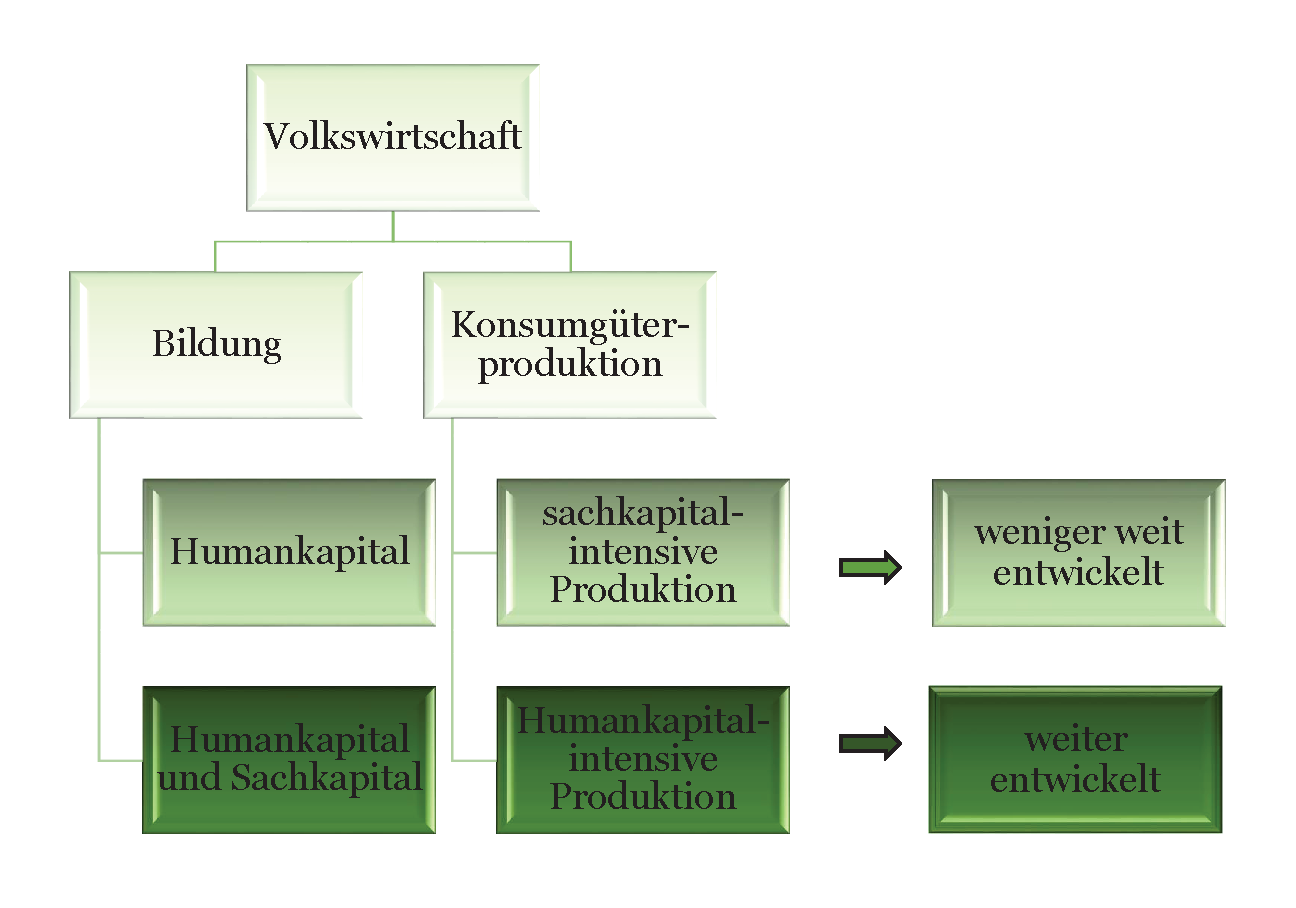
\includegraphics[width=0.7\textwidth]{C:/Users/BibiKiBa/Diss/Doktorarbeit/ModellEins/Abbildungen/SchemaPapierZwei.eps}
	\\
		\hfill\footnotesize\sffamily{\textbf{Quelle:}}  ENTWURF! eigene Darstellung
		\caption{Kategorisierung der Entwicklungsstufen}
		\label{fig:SchemaPapierZwei}		
\end{figure*}
In einer ökonomisch kleinen Volkswirtschaft gibt es die beiden Sektoren Güterproduktion und Bildung. Im Konsumgutsektor wird ein Gut produziert, hier die Handtasche, die einem repräsentativen Haushalt einen Nutzen stiftet. Der Nutzen besteht in diesem Fall aus der Bedürfnisbefriedigung etwas von einem Ort zu einem anderen transportieren zu können. Für die Herstellung des Gutes werden grundsätzlich physisches Kapital sowie auch Humankapital benötigt. Beide Produktionsfaktoren können jedoch gegeneinander substituiert werden und das Gut kann je nach Einsatzverhältnissen relativ sachkapitalintensiv oder humankapitalintensiv produziert werden. Auf das Beispiel bezogen bedeutet dies, dass eine Handtasche von speziell ausgebildeten Täschnern in Handarbeit hergestellt wird. Der Herstellungsprozess ist sehr aufwendig, detailorientiert und erfordert besondere Fähigkeiten und Fertigkeiten. Diese qualifizierte Arbeit ist sehr knapp und wird dementsprechend hochpreisig entlohnt. Ein konkretes Beispiel ist die in Frankreich gefertigte Birkin Bag der Marke Hermes, bei der weltweit nur wenige Menschen in der Lage sind diese mit den entsprechenden Qualitätsanforderungen herzustellen.\\
Jedoch kann eine Handtasche den gleichen Zweck erfüllen, wenn ihr Produktionsprozess durch weniger qualifizierte Arbeit und deutlich stärkeren Maschineneinsatz geprägt ist.
Ein Land wie beispielsweise Bangladesch, das spezialisiert ist auf die Textilindustrie, weist zwar eine relativ hohe Ausstattung an Arbeit vor, jedoch mit geringfügigeren Qualifikationen als Frankreich. Ein Gro{\ss}teil der arbeitenden Bevölkerung dieser Branche wird eine Industrienähmaschine bedienen können und auch weitere handwerkliche Fähigkeiten haben, jedoch sind die Arbeitsabläufe stark durch Arbeitsteilung geprägt und ein umsichtig allumfassender Überblick sowie eine fachkundige Einschätzung des Herstellungsprozesses fehlt. Der Schwerpunkt liegt dann auf der starken Spezialisierung jedes einzelnen Arbeiters auf einfache Arbeitsschritte, ohne dabei jedoch andere Fähigkeiten zu fördern. Somit können auch die Folgen und Konsequenzen einer Neuerung schlecht eingeschätzt werden. 
Neben der Unterscheidung des Produktionsprozesses im Konsumgütersektor wird auch der Bildungssektor hinsichtlich der Einsatzfaktoren differenziert. So besteht grundsätzlich die Möglichkeit nur durch den Einsatz von Lehrkräften, hier bereits ausgebildete Schneider, die Fähigkeiten auf weniger qualifizierte Arbeiter auszuweiten. 
Ebenfalls denkbar ist neben dem Einsatz von Lehrkräften ein zusätzlicher Einsatz von Sachkapital wie Nähmaschinen, Bücher oder Lehrvideos.\\
Auf Grundlage dieser Differenzierungsmöglichkeiten werden in diesem Kapitel verschiedene Entwicklungsstadien unterschieden. Demzufolge wird in einem relativ weniger weit entwickelten Land tendenziell mehr Sachkapital als Humankapital vorhanden sein und entsprechend die Produktionsstruktur diesem Umstand angepasst, also relativ sachkapitalintensiv produzieren. Hinzu kommt, dass meist auf den Einsatz von physischem Kapital im Bildungssektor verzichtet wird.\\
Bei einem relativ weiter entwickeltem Land wird angenommen, dass relativ gesehen mehr Humankapital als Sachkapital vorhanden ist, verglichen mit einem Land oder Region, das weniger weit entwickelt ist. Dies führt zu einer humankapitalintensiven Produktion im Konsumgutsektor und zu einer Optimierung des Bildungssektors durch den Einsatz beider Produktionsfaktoren. 

\section{Autarkie}
Zunächst wird die Situation ohne Handel betrachtet. Es wird ebenfalls ein zwei Sektor-Modell vorgestellt, dass sich noch stark an der Arbeit von \citet{Lucas.1988} orientiert. Bei dem einen Sektor handelt es sich um einen Konsum- bzw. Investitionsgutsektor bei dem anderen um den Bildungssektor.
\subsection*{Produktion}
In dem vorliegenden Modell einer geschlossenen Volkswirtschaft können die beiden Produktionsfaktoren physisches Kapital $K(t)$ und Arbeit $L(t)$ für den Konsumgut- oder Bildungssektor verwendet werden. 
Dabei wird angenommen, dass sich die Faktoren frei zwischen den beiden Sektoren bewegen können und demzufolge keine Anforderungen erfüllen müssen, um in den anderen Sektor zu wechseln. Die Mobilität der Faktoren führt zu einem Ausgleich der Faktorpreise \citep{Samuelson.1941}. Für physisches Kapital muss ein Zinssatz $r$ an die Kapitalgeber entrichtet werden und die Arbeiter erhalten den Lohnsatz $w$. Dabei ist der Preis für die Arbeit $w$ exogen gegeben und steigt nicht mit zusätzlicher Bildung an. Der Faktor Arbeit hängt von der Bevölkerungsgrö{\ss}e $N(t)$ eines Landes ab sowie vom durchschnittlichen Humankapitalbestand $h(t)$ und dem Anteil des Humankapitals $u(t)$, der in die Produktion des Konsumgutsektors eingeht.
\begin{equation}
L(t)=N(t)u(t)h(t)
\label{eq:Arbeit}
\end{equation}
Das physische Kapital setzt sich zusammen aus dem durchschnittlichen Kapitalbestand $k(t)$ und dem Anteil des physischen Kapitals $v(t)$, der ebenfalls bei der Produktion des Konsumgutes verwendet wird. 
\begin{equation}
K(t)=v(t)k(t)
\label{eq:Kapital}
\end{equation}
Die Produktionsfunktionen sind linear homogen und demnach liegen konstante Skalenerträge vor. Bei der Konsumgüterproduktion führt der erhöhte Einsatz von Produktionsfaktoren zu einem proportionalen Anstieg der Ausbringungsmenge.
\begin{equation}
\text{Konsumgutsektor:}\qquad F[K,L]= A(v(t)k(t))^\alpha(u(t)h(t))^{1-\alpha}
\label{eq:ProduktionsfunktionK}
\end{equation}
Das Gut kann abhängig von der Produktionselastizität $\alpha$ mit relativ viel physischem Kapital oder Humankapital produziert werden. Demnach kann die Handtasche durch vollständige Eigenleistung von qualifizierten Täschnern hergestellt werden, oder durch den verstärkten Einsatz von Maschinen bspw. während des Zuschneideprozesses.\\
Im Bildungssektor bedeutet konstante Skalenerträge, dass jede zusätzliche Einheit Bildung zu dem gleichen Lernerfolg führt.\footnote{Diese Annahme weicht insofern von der Realität ab, als das Bildung einen abnehmenden Grenzertrag aufweisen kann. Der zusätzliche Nutzen des "`Addierens"' und "`Subtrahierens"' ist höher als eine "`Wurzel ziehen"' zu können. Deshalb wird auf gesamtwirtschaftlicher Ebene weiterhin von abnehmenden Grenzerträgen ausgegangen, jedoch nicht auf der Ebene des Haushalts, der hier den Nutzen maximiert.} 
\begin{equation}
\text{Bildungssektor:} \qquad G[K,L]= B((1-v(t))k(t))^{\eta}((1-u(t))h(t))^{1-\eta}
\label{eq:ProduktionsfunktionH}
\end{equation}
Ebenso kann der Bildungssektor erweitert werden, durch den Einsatz von relativ viel physischem Kapital, wenn die Produktionselastizität $\eta$ hoch ist, oder eher humankapitalintensiv, wenn $\eta$ gering ist. Auch im Lernprozess spielt das Einsatzverhältnis eine Rolle. Angenommen es wird einer Gruppe von Schneiderlehrlingen durch die Lehrkraft an einem Beispiel mit nur einer Nähmaschine ein Prozess vorgeführt, ist der Lernerfolg ein anderer, als wenn jeder einzelne die Möglichkeit hat an einer eigenen Nähmaschine die neue Technik beliebig oft zu wiederholen und zu üben.  \\
Die Aufteilung der Produktionsfaktoren auf die Sektoren wird dargestellt durch die Anteile $u(t)$ bzw. $v(t)$. Das physische Kapital wird im Konsumsektor verwendet mit $v(t)$ und im Bildungssektor mit $(1-v(t))$. Um das Beispiel der Textilindustrie aufzugreifen, wäre physisches Kapital bei der Produktion einer Handtasche die Nadel, bzw. die Nähmaschine. Dieses kann entweder dazu verwendet werden tatsächlich Güter zu produzieren, oder aber um die Qualifikationen zu erweitern und den Lernprozess zu beschleunigen, indem man das neu gewonnene Wissen direkt anwendet. Ganz ähnlich erfolgt die Aufteilung des Humankapitals. Der Anteil $u(t)$ des Humankapitals wird für die Herstellung des Konsumgutes eingesetzt, wohingegen $(1-u(t))$  in den Bildungssektor eingeht. Auch hier kann das Wissen eines Einzelnen über die Zuschnitttechniken oder Säuberungsarbeiten  bei der Herstellung des Gutes eingesetzt werden, oder als Multiplikator im Bildungssektor, indem das vorhandene Wissen an bislang Unwissende weiter getragen wird.
\subsection*{Konsum}
Die Gesamtheit aller Haushalte richtet sich nach der Bevölkerungsgrö{\ss}e eines Landes, die mit der exogenen Rate $n$ über die Zeit $t$ wächst und von der anfänglichen Bevölkerungsgrö{\ss}e $N_0$ ausgeht.  
\begin{equation}
N(t)=N_0e^{nt}
\label{eq:Bevolkerungsentwickung}
\end{equation}
Die von den Unternehmen nachgefragten Produktionsfaktoren physisches Kapital und Humankapital bieten die Haushalte über die Faktormärkte an. Sie haben die Wahl die Konsumgüter zu verbrauchen oder diese in zukünftigen Konsum zu investieren, also zu sparen und dadurch Kapital zu akkumulieren. 
Es wird angenommen, dass alle Haushalte die gleichen Präferenzen haben und sie ihren Nutzen intertemporal maximieren. Auch hier wird von der Symmetrie der Haushalte ausgegangen und sie diskontieren ihren zukünftigen Nutzen mit der gleichen Rate, $\rho$. Der zukünftige Nutzen ist ihnen weniger wert, als der heutige Nutzen, demnach gilt, dass $\rho>0$. 
\begin{equation}
V=\int \limits_{0}^\infty  \! e^{-\rho t}\psi(c(t)) \, dt
\end{equation}
Der angeführte Lebenszeitnutzen $V$ bei einem unendlichen Zeithorizont ergibt sich aus der Gesamtheit aller jeweils gegenwärtigen Nutzenwerte zu den verschiedenen Zeitpunkten. Die Zeitpunkte sind additiv separabel miteinander verknüpft. Demnach wird der aus dem Konsum resultierende Nutzen in jedem Zeitpunkt neu bewertet und wird unabhängig von der Bewertung zu einem anderen Zeitpunkt sein.
\begin{equation}
\psi(c(t))=\frac{c(t)^{1-\sigma}}{1-\sigma}
\end{equation} 
Der gegenwärtige Nutzen der Haushalte $\psi(t)$ ist nur von der konsumierten Menge der Güter $c(t)$ abhängig, nicht vom Bildungsniveau. Au{\ss}erdem ist der Konsum zwischen den Zeitpunkten intertemporal variabel, in welchem Ausma{\ss} der Konsum zwischen zwei Zeitpunkten substituiert werden kann, hängt von der intertemporalen Substitutionselastizität $\sigma$ ab.\\
Die Maximierung des intertemporalen Nutzens lässt die Haushalte einen optimalen Konsumpfad wählen. Dabei müssen sie sich entscheiden zwischen dem Konsum  des Gutes oder der Investition in den Kapitalstock. Hinzu kommen die Entscheidungen hinsichtlich der Aufteilung des physischen Kapitals und Humankapitals auf die beiden Sektoren, welche Aussagen über die Präferenzen der Haushalte, bezüglich des Konsums und der Bildung zulässt. Demzufolge sind die Entscheidungsvariablen des folgenden Maximierungsproblems die Konsummenge $c(t)$, der Anteil des physischen Kapitals, der in die Produktion des Konsumgutes eingeht $v(t)$ und darüber gleichzeitig den Humankapitalsektor determiniert, wegen $(1-v(t))$, sowie der Aufteilung des Humankapitals durch $u(t)$ auf die beiden Sektoren.\\
Die dynamische Betrachtung des zu maximierenden Lebenszeitnutzens $V$ verläuft über den Zeithorizont von $0$ bis $\infty$ und beginnt mit den Anfangswerten des Kapitals $k_0$ und $h_0$.\footnote{Die beiden Startwerte $k_0$ und $h_0$ sind exogen.}
\begin{equation}\operatorname*{max}_{c(t),u(t),v(t)}V[k_0,h_0]= \int_{0}^\infty e^{-\rho t} \frac{c(t)^{1-\sigma}}{1-\sigma}dt\end{equation}
Der Nutzen wird nur dann maximal, wenn die beiden Veränderungen der Kapitalstöcke über die Zeit berücksichtigt werden. Denn durch jede zusätzliche Einheit Kapital verändert sich der Lebenszeitnutzen. Durch einen gegenwärtigen Aufbau eines Kapitalstocks kann zukünftig mehr Nutzen generiert werden. Es besteht also eine direkte Abhängigkeit zwischen den Bewegungsgleichungen von Sach- und Humankapital, $\dot{k}$ und $\dot{h}$, sowie dem Lebenszeitnutzen.
		\begin{equation}\dot{k}(t)=A(v(t)k(t))^\alpha(u(t)h(t))^{1-\alpha}-c(t)\end{equation}\vspace{-0.8cm}
		\begin{equation} \dot{h}(t)=B((1-v(t))k(t))^{\eta}((1-u(t))h(t))^{1-\eta}\end{equation}
		\vspace{-0.3cm}
		\begin{displaymath} c(t)\geq 0,\quad k(t)\geq 0,\quad h(t)\geq 0, \end{displaymath}
		\begin{displaymath} 0\leq u(t)\leq 1,\quad 0\leq v(t) \leq1, \end{displaymath}
		\begin{displaymath} 0\leq \alpha\leq 1,\quad 0\leq \eta \leq1, \quad A\geq 0, \quad B\geq 0\end{displaymath}
Das Sachkapital erhöht sich durch all die produzierten Güter, die nicht konsumiert werden. Der Produktion der Güter dient sowohl physisches Kapital als auch Humankapital. Bei $A$ handelt es sich um einen Technologieparameter, der das technische Wissen im Konsumgutsektor berücksichtigt. Humankapital wird ebenfalls durch beide Kapitalarten aufgebaut und durch den Technologieparameter $B$ beeinflusst. Dabei gehen die Produktionsfaktoren jeweils mit einer Produktionselastizität von $\alpha$ bzw. $\eta$ in den jeweiligen Prozess ein.\\
Da es sich um ein intertemporales Optimierungsproblem handelt, ist es mit der Hamilton Funktion zu lösen. Dieses Verfahren wird auch Maximumprinzip genannt und geht zurück auf \citep{Pontryagin.1964}. Es beschreibt den optimalen Konsumpfad, der den Lebenszeitnutzen, unter Berücksichtigung der Entscheidungen der Haushalte über $c(t)$, $u(t)$ und $v(t)$ maximiert. Diese Entscheidungsvariablen determinieren die zukünftige Ausweitung der Kapitalstöcke $k(t)$ und $h(t)$. Es besteht zu jedem Zeitpunkt eine Abhängigkeit des Lebenszeitnutzens zu dem jeweils gegenwärtig vorhandenem physischen Kapitalstock und Humankapitalstock, sowie zu den Entscheidungen des Haushalts über die Aufteilung der Ressourcen auf die beiden Sektoren.\footnote{Ressourccen eines Haushalts können die Zeit, Kraft oder auch die Konzentration sein.} Deshalb sind für die Lösung des dynamischen Maximierungsproblems die Bewegungsgleichungen von $h(t)$ und $k(t)$ notwendig, da diese die jeweilige Veränderung der Kapitalstöcke über die Zeit beschreiben.\footnote{Aus Gründen der Anschaulichkeit wird im folgenden die Abhängigkeit der Variablen gegenüber der Zeit $t$ vernachlässigt.}
\begin{equation}
\begin{split}
\mathbb{H}=&~e^{-\rho t}\frac{c^{1-\sigma}}{1-\sigma}\\
&+\gamma_1(A(vk)^\alpha(uh)^{1-\alpha}-c)\\
&+\gamma_2B[(1-v)k]^{\eta}[(1-u)h]^{1-\eta}\\
\end{split}
\end{equation}
\begin{displaymath} \gamma_1 > 0,\quad \gamma_2 > 0 \end{displaymath}
Die Optimierung über die Hamiltonfunktion gibt Auskunft über den resultierenden Gesamtnutzen für die anberaumte Lebenszeit. Au{\ss}erdem ist ein Vergleich resultierender Nutzwerte zweier aufeinanderfolgender Zeitpunkte möglich. Der erste Summand beschreibt den gegenwärtigen Nutzeneffekt herbeigeführt durch den Konsum von Gütern, der wiederum über die Entscheidungsvariablen determineirt wird. Die folgenden Summanden der Hamiltonian stellen die zukünftigen Nutzeneffekte der zukünftigen Veränderungen des Sach- und Humankapitals dar, dessen gegenwärtige Nutzwerte durch die zugeh{\"o}rigen Schattenpreise $\gamma_1$ und $\gamma_2$ ausgedrückt werden.\footnote{Bei den Variablen $\gamma_1$ und $\gamma_2$ handelt es sich originär um Hilfsvariablen oder auch als Schlupfvariablen bekannt, die hier als Schattenpreis interpretiert werden können.} Die Schattenpreise ergeben sich aus der Ableitung des Lebenszeitnutzens nach jeweils einem Produktionsfaktor und sind somit der Lebenszeitgrenznutzen einer Einheit Sach- oder Humankapital. Dieser drückt den Wert einer zusätzlichen Einheit Kapital für den gesamten Zeithorizont aus, also eine mögliche marginale Lebenszeitnutzenverbesserung durch eine zusätzliche Einheit Kapital.  Beide Schattenpreise sind positiv, da ansonsten eine Einsatzfaktoränderung zu einer Indifferenz der Haushalte führt. Denn bei einem Schattenpreis von Null würde der zukünftige Nutzen den Lebenszeitnutzen nicht tangieren und der Fokus auf der Gegenwart liegen ohne zukünftige Zeitpunkte zu berücksichtigen. Durch die Multiplikation mit dem Schattenpreis wird der Nutzwert der Kapitalerhöhung berücksichtigt. Der Schattenpreis "`konvertiert"' die Faktoreinheiten in Nutzeinheiten unter Berücksichtigung der zeitlichen Veränderung. Beide Nutzeneffekte konkurrieren miteinander, da ein gegenwärtiger Konsum den zukünftigen mindert \citep{Chiang.2000,Chiang.2011}.\\   
Diese Optimierung findet für alle möglichen Zeitpunkte statt und ermöglicht eine Vergleichbarkeit zweier aufeinanderfolgender Zeitpunkte. Erst dann wenn der heutige Grenznutzen mit dem morgigen übereinstimmt, wurde der optimale Konsumpfad einer Volkswirtschaft gefunden \citep{Chiang.2000}. Folgende Bedingungen erster Ordnung lösen das Optimierungsproblem.\footnote{Die ausführliche Berechnung aller Gleichgewichtsbedingungen sind in Appendix \ref{AutarkieAPPENDIX} zu finden.}  
\begin{align}
&\frac{\partial\mathbb{H}}{\partial c}\overset{!}{=}~0\label{eq:foc1WM}\\
&\frac{\partial\mathbb{H}}{\partial v}\overset{!}{=}~0\label{eq:foc2WM}\\
&\frac{\partial\mathbb{H}}{\partial k}\overset{!}{=}-\dot{\gamma_1}\label{eq:foc3WM}\\
&\frac{\partial\mathbb{H}}{\partial u}\overset{!}{=}~0\label{eq:foc4WM}\\
&\frac{\partial\mathbb{H}}{\partial h}\overset{!}{=}-\dot{\gamma_2}\label{eq:foc5WM}\end{align}
Die Bedingungen erster Ordnung werden im Folgenden recht allgemein, jedoch sehr ausführlich beschrieben, um in der folgenden Analyse hinsichtlich verschiedener Entwicklungsstände grö{\ss}tenteils darauf verzichten zu können. 
\subsubsection*{Ableitung nach Zustandsvariablen, $k$ und $h$}
Die Ableitung nach einer Zustandsvariablen wird mit der jeweiligen negativen Bewegungsgleichung des Schattenpreises gleichgesetzt.\footnote{Der Lebenszeitgrenznutzen einer zusätzlichen Einheit $\gamma$ ist zwar positiv, jedoch abnehmend mit zunehmendem Kapitaleinsatz über die Zeit. Demzufolge ist die Ableitung des Schattenpreises nach der Zeit negativ. Das negative Vorzeichen gleicht diesen Zusammenhang aus und es kann eine Gleichheit beider Seiten herbeigeführt werden.} Dabei handelt es sich um eine intertemporale Arbitragebedingung, die gleich dem jeweiligen negativen Lebenszeitgrenznutzen sein soll. Die Abnahme des Schattenpreises über die Zeit $\dot{\gamma}$ kann auch als Abschreibungsrate des Schattenpreises interpretiert werden und soll genau so gro{\ss} sein, wie die Erhöhung des gegenwärtigen und zukünftigen Nutzen durch die Kapitalakkumulation. Erst wenn sich beide Grö{\ss}en ausgeglichen haben, kann der Lebenszeitnutzen maximal sein \citep{Chiang.2000,Chiang.2011}.

\subsubsection*{Ableitung nach Entscheidungsvariablen $v$,$u$ und $c$ }
Die Ableitung nach einer Zustandsvariablen ergibt die optimale Allokation eines Produktionsfaktors in jedem Sektor zu jedem Zeitpunkt. Die Gleichsetzung der Ableitung einer Entscheidungsvariablen mit $0$ bedeutet, dass dann diese Variable maximal sein wird, unter der Voraussetzung, dass die Bedingung der jeweils zugehörigen Zustandsvariablen erf{\"u}llt ist.\newline 
Die Entscheidungsvariable wird direkt vom Wirtschaftssubjekt gewählt, aus ihr ergibt sich dann indirekt die Zustandsvariable \citep{Chiang.2011}. Die Haushalte entscheiden sich sowohl für den Konsum, als auch für die Aufteilung der eigenen Ressourcen, die ihren Nutzen maximieren. Dabei muss, um beim anfänglichen Beispiel zu bleiben, berücksichtigt werden, wie viele Handtaschen sie derzeit konsumieren möchten und wie viel Sachkapital, wie Nadeln, Nähmaschinen oder Scheren  sie bereit sind für die Produktion bzw. für ihre Weiterbildung zu den unterschiedlichen Zeitpunkten zu investieren. 

\subsubsection*{Ableitung nach $c$}
Durch die Ableitung der Hamiltonian nach dem Konsum $c$, siehe \colorbox{lightgray}{Gleichung \eqref{eq:foc1WM}}, wird der maximale Konsum unter Ber{\"u}cksichtigung der Nebenbedingungen $\dot{k}$ und $\dot{h}$ bestimmt.
\begin{equation}
\colorbox{lightgray}{$\partial\mathbb{H}/\partial c\overset{!}{=}~0$}
\end{equation}
\vspace{-0.5cm}
\begin{equation}
e^{-\rho t}c^{-\sigma}-\gamma_1 = 0
\end{equation}
\vspace{-0.7cm}
\begin{equation}
\gamma_1=e^{-\rho t}c^{-\sigma}
\label{eq:foc1WMa}
\end{equation}
Die Gleichung \eqref{eq:foc1WMa} dr{\"u}ckt aus, dass der diskontierte Grenznutzen des optimalen Konsums pro Kopf gleich dem gegenwärtigen Schattenpreis $\gamma_1$ einer zusätzlichen Sachkapitaleinheit ist. Da auch die zweite Ableitung nach $c$ kleiner $0$ ist, handelt es sich um einen maximalen Punkt. 
\begin{equation}
-e^{-\rho t}\sigma c^{-\sigma-1}<0
\end{equation}
Der Schattenpreis beschreibt in diesem Fall wie hoch die Lebenszeitnutzenerhöhung ist, wenn auf den heutigen Konsum verzichtet wird und welchen zukünftigen Nutzenwert die  daraus resultierende Kapitalakkumulation stiften wird.\\
Die optimale Konsumgütermenge beeinflusst im Wesentlichen die Sachkapitalakkumulation. Die Entscheidung des Haushalts über die gegenwärtige Konsummenge an Handtaschen bedingt die Akkumulation von Handtaschen und den damit verbundenen Güterberg. Denn je mehr konsumiert wird, desto weniger Gütereinheiten können in die Kapitalakkumulation investiert werden. Demzufolge ist für die weitere Analyse eine Ableitung der Zustandsvariablen $k$ notwendig.
 
\subsubsection*{Ableitung nach $k$}
Bei der Variablen $k$ handelt es sich um eine Zustandsvariable, die den aus der Konsumentscheidung resultierenden Zustand angibt. Neben dem Konsum beeinflusst auch die Aufteilung des Sachkapitals auf die beiden Sektoren $v$ den Kapitalbestand. Steigt der Kapitalstock um eine Einheit an, dann erhöht sich der Lebenszeitnutzen um den Schattenpreis, der den Wert dieser zusätzlichen Kapitaleinheit in Nutzeneinheiten angibt. Diese Auswirkung auf den Nutzen durch die Veränderung einer Einheit Sachkapital beschreibt \colorbox{lightgray}{Gleichung \eqref{eq:foc3WM}}. Der gegenwärtige Grenznutzen des physischen Kapitals soll also dem zukünftigen Nutzen einer Einheit Sachkapital entsprechen. Der Einsatz einer zusätzlichen Nähmaschine führt im Konsumgütersektor zu einer erhöhten Produktion von Handtaschen, die entweder für den Eigenbedarf genutzt werden können oder aber den Kapitalstock erhöhen. Es besteht jedoch auch die Möglichkeit die Sachkapitaleinheit in den Bildungssektor für das Erlernen neuer effizienterer Nähtechniken zu investieren. In beiden Fällen erhöht sich der Lebenszeitnutzen, entweder durch den gegenwärtigen oder durch den zukünftigen Konsum. Die Höhe des zusätzlichen künftigen Nutzens wird am Schattenpreis bemessen. So gilt f{\"u}r die erste Ableitung der Hamiltonian nach dem physischen Kapital $k$, dass diese im Gleichgewicht der negativen ersten Ableitung nach der Zeit des Schattenpreises von Sachkapital entspricht. 
\begin{equation}
\colorbox{lightgray}{$\partial\mathbb{H}/\partial k\overset{!}{=}-\dot{\gamma_1}$}\label{nachK}
\end{equation}
\begin{equation}
\gamma_{1}A v^{\alpha}k^{\alpha -1} \alpha(u h)^{1- \alpha} + \gamma_{2}B(1- v)^{\eta} k^{\eta -1} \eta \left [ (1-u)h \right ]^{1- \eta}\overset{!}{=} - \dot{\gamma}_{1}\label{BedingungFoc3WM}
\end{equation}

Der gegenwärtige Nutzwert der auf Human- und Sachkapitalakkumulation zurückzuführen ist, soll dem zukünftigen Nutzwert entsprechen. Der Schattenpreis $\gamma_1$ wird mit der Rate abgeschrieben, mit der die künftige Kapitalakkumulation zur Lebenszeitnutzenerhöhung beiträgt. Erst wenn diese Bedingung erfüllt ist kann der Nutzen maximal sein \citep{Chiang.2000}.

\subsubsection*{Ableitung nach $v$}
Bei der Aufteilung des Sachkapitals den Konsumgutsektor und den Bildungssektor $v$, handelt es sich ebenfalls um eine Entscheidungsvariable. Indem eine marginale Veränderung dieser Aufteilung auf den Nutzen gleich null gesetzt wird, kann der Nutzen maximiert werden, sofern die Bedingung gemä{\ss} Gleichung \eqref{BedingungFoc3WM} erfüllt ist.
Wird die allgemeine Form aus \colorbox{lightgray}{Gleichung \eqref{eq:foc2WM}} hier konkret ausformuliert ergibt sich:
\begin{equation}
\colorbox{lightgray}{$\partial\mathbb{H}/\partial v\overset{!}{=}~0$}
\end{equation}
\vspace{-0.5cm}
\begin{equation}
\gamma_1A\alpha v^{\alpha-1}k^\alpha(uh)^{1-\alpha}-\gamma_2B\eta(1-v)^{\eta-1}k^\eta[(1-u)h]^{1-\eta}\overset{!}{=}~0
\end{equation}
\vspace{-0.7cm}
\begin{equation}
\gamma_1A\alpha v^{\alpha-1}k^\alpha(uh)^{1-\alpha}=\gamma_2B\eta(1-v)^{\eta-1}k^\eta[(1-u)h]^{1-\eta}
\end{equation}
Demzufolge sollen sich die mit dem Schattenpreis bewerteten Grenzprodukte entsprechen. Eine zukünftige marginale Veränderung von $u$ bedingt im Konsumgutsektor einen anteilig höheren Einsatz von Sachkapital um den der Anteil im Bildungssektor dadurch reduziert wird. Der resultierende zusätzliche Nutzen des Kapitaleinsatzes im Konsumgutsektor soll die Minderung des Nutzens im Bildungssektor ausgleichen. Durch den Einsatz einer Nähmaschine in der Textilindustrie kommt es zu einer Nutzensteigerung, die genau der Nutzenminderung im Bildungssektor entsprechen muss. 

\subsubsection*{Ableitung nach $h$}
Auch im Bildungssektor soll sich die Veränderung der Lebenszeitgrenznutzen zweier aufeinanderfolgender Perioden entsprechen. Diesen Zusammenhang beschreibt \colorbox{lightgray}{Gleichung \eqref{eq:foc5WM}}. Der Grenznutzen des Humankapitals beschreibt eine Veränderung der Hamiltonian durch einen Anstieg um eine Einheit Humankapital und soll heute genau soviel Nutzen stiften wie in der folgenden Periode.
\begin{equation}
\colorbox{lightgray}{$\partial\mathbb{H}/\partial h\overset{!}{=}-\dot{\gamma_2}$}\label{nachH}
\end{equation}
\begin{equation}
\gamma_1A(1-\alpha)(vk)^\alpha u^{1-\alpha}h^{-\alpha}+\gamma_2 B(1-\eta)[(1-v)k]^{\eta}(1-u)^{1-\eta}h^{-\eta}\overset{!}{=}-\dot{\gamma}_2\label{GNHK}
\end{equation}
Dies ist genau dann erfüllt, wenn der zukünftige Nutzenwert der zusätzlichen Humankapitaleinheit dem heutigen Grenznutzen entspricht, da der Schattenpreis mit einer Rate von $-\gamma_2$ abgeschrieben wird. Der gegenwärtige Nutzengewinn aus einer Einheit qualifizierter Arbeit entspricht dem zukünftigen Nutzen durch den Einsatz selbiger in den Bildungssektor. Es sollte demnach im Gleichgewicht keinen Unterschied machen, wann ein ausgebildeter Schneider eingesetzt wird. 

\subsubsection*{Ableitung nach $u$}
Ist die Bedingung \eqref{GNHK} erfüllt, dann kann $u$ so gewählt werden, dass die Hamiltonian zu jedem Zeitpunkt maximal ist, indem \colorbox{lightgray}{Gleichung \eqref{eq:foc4WM}} gilt.
\begin{equation}
\colorbox{lightgray}{$\partial\mathbb{H}/\partial u\overset{!}{=}~0$}
\end{equation}
\vspace{-0.5cm}
\begin{equation}
\gamma_1A(1-\alpha)(vk)^{\alpha}h^{1-\alpha}u^{-\alpha}-\gamma_2B(1-\eta)[(1-v)k]^\eta (1-u)^{-\eta} h^{1-\eta}\overset{!}{=}0
\end{equation}
\vspace{-0.7cm}
\begin{equation}
\gamma_1A(1-\alpha)(vk)^{\alpha}h^{1-\alpha}u^{-\alpha}=\gamma_2B(1-\eta)[(1-v)k]^\eta (1-u)^{-\eta} h^{1-\eta}\label{foc4}
\end{equation}
Die Aufteilung führt zu einem maximalen Nutzen, wenn sich die zukünftigen Grenzprodukte beider Sektoren entsprechen. Eine Umverteilung des Humankapitals muss in beiden Sektoren die gleiche Nutzenveränderung herbeirufen. Dann verändert sich der Lebenszeitnutzen nicht mehr durch eine Umverteilung des Einsatzortes des ausgebildeten Täschners.

\subsubsection*{Transversalitätsbedingung}
Die Transversalitätsbedingungen sind begrenzende Bedingungen der Schattenpreise. Sie gewährleisten, dass zum angenommen Endzeitpunkt des geplanten Zeithorizonts der Bestand der Zustandsvariablen vollständig aufgebraucht oder deren Wert in Höhe der Schattenpreise zum Planungsendzeitpunkt gleich $0$ ist \citep{Chiang.2000}.
%Sie beschreiben den Zeithorizont der zu treffenden Entscheidungen, hier über den Konsum, die Aufteilung des physisches Kapital und Humankapitals auf die beiden Sektoren.
\begin{equation} \lim_{t \to \infty}e^{-\rho t}\gamma_1k=0\end{equation}
\vspace{-0.7cm}
\begin{equation} \lim_{t \to \infty}e^{-\rho t}\gamma_2h=0\end{equation}

\subsection*{Gleichgewichtsbedingungen}
Fasst man die zuvor separat erläuterten Bedingungen zusammen, dann ergibt sich ein Gleichungssystem, welches die notwendigen Bedingungen beschreibt, damit eine autarke Volkswirtschaft langfristig im Gleichgewicht ist. 
\begin{align}
&\gamma_1=e^{-\rho t}c^{-\sigma}\\
&\gamma_1A\alpha v^{\alpha-1}k^\alpha(uh)^{1-\alpha}=\gamma_2B\eta(1-v)^{\eta-1}k^\eta[(1-u)h]^{1-\eta}\\
&\gamma_{1}A v^{\alpha}k^{\alpha -1} \alpha(u h)^{1- \alpha} + \gamma_{2}B(1- v)^{\eta} k^{\eta -1} \eta \left [ (1-u)h \right ]^{1- \eta}= - \dot{\gamma}_{1}\label{foc3IL}\\
&\gamma_1A(1-\alpha)(vk)^{\alpha}h^{1-\alpha}u^{-\alpha}=\gamma_2B(1-\eta)[(1-v)k]^\eta (1-u)^{-\eta} h^{1-\eta}\\
&\gamma_1A(1-\alpha)(vk)^\alpha u^{1-\alpha}h^{-\alpha}+\gamma_2 B(1-\eta)[(1-v)k]^{\eta}(1-u)^{1-\eta}h^{-\eta}=-\dot{\gamma}_2
\end{align}
\vspace{-0.7cm}
\begin{equation} \lim_{t \to \infty}e^{-\rho t}\gamma_1k=0\end{equation}
\vspace{-0.7cm}
\begin{equation} \lim_{t \to \infty}e^{-\rho t}\gamma_2h=0\end{equation}
Aus diesen Bedingungen lässt sich, wie in Appendix \ref{AutarkieAPPENDIX} dargestellt, das gleichgewichtige Wachstum herleiten. 

\subsubsection*{Keynes-Ramsey-Regel}
Die Keynes-Ramsey-Regel beschreibt in ihrer ursprünglichen Form die Beziehung zwischen dem Grenzprodukt des Kapitals und dem daraus resultierenden Wirtschaftswachstum.  
\begin{equation}
\boxed{\hat{c}=\frac{1}{\sigma}\left(A\alpha \left(\frac{vk}{uh}\right)^{\alpha -1}-\rho\right)}\label{KRRWM}
\end{equation}
Je produktiver eine Einheit Sachkapital ist, desto höher ist die Wachstumsrate. Es besteht ein positiver Zusammenhang zwischen dem Grenzprodukt des physischen Kapitals $A\alpha \left(\frac{vk}{uh}\right)^{\alpha -1}$ und der Wachstumsrate. Wohingegen ein negativer bzw. inverser Zusammenhang zwischen selbiger Wachstumsrate und dem Diskontfaktor $\rho$ besteht.\footnote{Der Kehrwert der intertemporalen Substitutionselastizität $1/\sigma$ ist ebenfalls positiv mit der Wachstumsrate verknüpft. Je leichter man zwischen den Zeitpunkten substituieren kann, desto höher ist die Wachstumsrate.} 
Diese Gleichung lässt jedoch noch keine konkreten Aussagen über die tatsächliche Grö{\ss}e der Variablen zu. So ist noch immer unklar wie hoch $u$ oder auch $v$ gewählt werden muss, um zum gleichgewichtigen Wachstumspfad zu konvergieren. Ebenso verhält es sich mit den Zustandsvariablen $k$ und $h$, auch hier ist noch unbekannt wie gro{\ss} diese im Gleichgewicht sind. Die Gleichgewichtswerte werden im folgenden Abschnitt \nameref{sec:Modelldynamik} beschrieben, deren Berechnung ist ausführlich in Appendix \ref{AutarkieAPPENDIX} zu finden. 

\subsection*{Modelldynamik}\label{sec:Modelldynamik}
Gleichung \eqref{KRRWM} zeigt, wenn das Verhältnis $k/h$ und die Kapitalaufteilungen $u$ und $v$ konstant sind, dass dann der Konsum mit konstanter Rate wächst. 
Betrachtet man das Wachstum des physischen Kapitals, dann sind ebenfalls das Verhältnis beider Kapitalarten $k/h$ sowie die Aufteilungen $v$ und $u$ relevant. Hinzu kommt das Verhältnis des Konsums zum physischen Kapital $c/k$ bzw. $\chi$.\footnote{Ersetzt man $\chi=\frac{c}{k}$ ergeben sich zwei Schreibweisen für die Wachstumsrate des physischen Kapitals.} Erst wenn diese konstant sind, wächst das Sachkapital $k$ mit konstanter Rate.
\begin{equation}
\hat{k}=Av^\alpha k^{\alpha-1}(uh)^{1-\alpha}-\frac{c}{k} \qquad \hat{=} \qquad
\hat{k}=Av^\alpha k^{\alpha-1}(uh)^{1-\alpha}-\chi 
\end{equation}
Ganz ähnlich verhält es sich mit dem Humankapital. Hier müssen wieder $k/h$, $v$ und $u$ konstant sein, damit das Humankapitalwachstum konstant ist. 
\begin{equation}
\hat{h}=B\left[(1-v)\frac{k}{h}\right]^{\eta}(1-u)^{1-\eta}
\end{equation}
Verkürzt durch $x_1=\frac{vk}{uh}$ und $x_2=\frac{(1-v)k}{(1-u)h}$ lassen sich diese Gleichungen auch schreiben als:
\begin{equation}
\boxed{\hat{k}=Ax_1^\alpha \frac{uh}{k}-\chi}
\end{equation}
\begin{equation}
\boxed{\hat{h}=Bx_2^\eta(1-u)}
\end{equation}
Es liegt nahe, dass im Steady-State gilt, dass $\hat{c}=\hat{k}=\hat{h}$ und somit die Wachstumsraten gleich gro{\ss} sind, wenn $k/h$, $c/k$, $u$ und $v$ konstante Grö{\ss}en sind. 

Eine Volkswirtschaft befindet sich dann im Gleichgewicht, wenn sich die Verhältnisse der Grenzproduktivitäten beider Sektoren entsprechen, die sich aus den Gleichungen \eqref{eq:foc2WM} und \eqref{eq:foc3WM} herleiten lassen. Eine Umverteilung des Kapitals zwischen den Sektoren stellt im Gleichgewicht keinen Sektor besser als zuvor. 
\begin{equation}
\boxed{\frac{1-\alpha}{\alpha}x_1=\frac{1-\eta}{\eta}x_2}
\end{equation}
Eine zusätzliche Sach- oder Humankapitaleinheit weist im Konsumgutsektor die gleiche Grenzproduktivität auf wie im Bildungssektor. Dies ist dann der Fall, wenn sich die Schattenpreisverhältnisse in beiden Sektoren entsprechen und somit das Verhältnis der Lebenszeitgrenznutzen in beiden gleich gro{\ss} ist. Langfristig verhalten sich die Relationen $x_1$ und $x_2$ gleich und mit Hilfe der folgenden Gleichung \eqref{A5} können die Wachstumsraten $\hat{x}_1$ und $\hat{x}_2$ berechnet werden, die demnach im Gleichgewicht konstant sind. 
\begin{equation}
\hat{x}_1=\hat{x}_2=0
\end{equation}
Zur Lösung des Gleichungssystems ist eine weitere Bedingung notwendig, die sich aus Gleichung \eqref{nachK} und \eqref{nachH} herleiten lässt. Diese drücken aus, dass zum einen die Rate des Lebenszeitgrenznutzens von Humankapital dem Grenzprodukt des Humankapitals entspricht. Zum anderen die Wachstumsrate des Schattenpreises des physischen Kapitals ebenso gleich dem Grenzprodukt des Kapitals im Konsumgutsektor ist. 
\begin{equation}
\boxed{B(1-\eta)x_2^\eta=-\rho-\sigma\hat{c}-\alpha\hat{x}_1+\eta\hat{x}_2}\label{A5}
\end{equation}
Der Nutzen aus einer zusätzlichen Humankapitaleinheit im Bildungssektor ist gleich dem resultierenden Nutzen einer zusätzlichen Einheit Sachkapital, da $\rho-\sigma\hat{c}=\hat{\gamma_1}=-A\alpha x_1^{\alpha-1}$ gemä{\ss} Gleichung \eqref{foc3IL}.
Demzufolge ergibt sich folgendes Gleichungssystem, welches das Gleichgewicht beschreibt. 
\begin{align}
&\hat{k}=Ax_1^\alpha \frac{uh}{k}-\chi\label{GG1WM}\\
&\hat{h}=Bx_2^\eta(1-u)\label{GG2WM}\\
& x_1(1-\alpha)/\alpha =x_2(1-\eta)/\eta\label{GG3WM}\\
&\hat{c}=\frac{1}{\sigma}\left(A\alpha x_1^{\alpha -1}-\rho\right)\label{GG4WM}\\
&B(1-\eta)x_2^\eta=-\rho-\sigma\hat{c}-\alpha\hat{x}_1+\eta\hat{x}_2\label{GG5WM}
\end{align}
Mithilfe dieses Gleichungssystems können die gleichgewichtigen Werte der verschiedenen Variablen bestimmt werden. Durch die Auflösung nach den optimalen Werten für $x_1$ und $x_2$ wird die Konsumwachstumsrate umgeformt in:\footnote{Siehe Appendix \ref{AutarkieAPPENDIX}.} 
\begin{equation}
\boxed{\hat{c}^*=\frac{1}{\sigma}\left(\left[A^\eta\alpha^{\alpha\eta}(1-\eta)^{(1-\eta)(1-\alpha)}(\eta(1-\alpha))^{\eta(1-\alpha)}B^{1-\alpha}\right]^\frac{1}{1+\eta-\alpha}-\rho\right)}
\end{equation}
Dabei hängt das Grenzprodukt $\left[A^\eta\alpha^{\alpha\eta}(1-\eta)^{(1-\eta)(1-\alpha)}(\eta(1-\alpha))^{\eta(1-\alpha)}B^{1-\alpha}\right]^\frac{1}{1+\eta-\alpha}$ von den Technologieparametern $A$ und $B$ beider Sektoren ab und wird im folgenden mit $M$ abgekürzt. Durch jeglichen technologischen Fortschritt erhöht sich das Wirtschaftswachstum.\\
Die gleichgewichtige Aufteilung des Humankapitals $u^*$ ist dadurch bedingt, dass im Gleichgewicht \colorbox{lightgray}{$\hat{c}=\hat{h}$} gilt.
\begin{equation}
\boxed{u^*=\frac{\sigma M-(1-\eta)(M-\rho)}{\sigma M}}\label{uOptAut}
\end{equation}
Im wesentlichen existiert eine Abhängigkeit der Humankapitalaufteilung $u$ zum Grenzprodukt des Kapitals $M$. Zwischen beiden besteht eine inverse Beziehung, somit wird ein abnehmendes Grenzprodukt des Kapitals durch den erhöhten Einsatz von Humankapital in den Konsumgutsektor kompensiert. Wenn jede zusätzliche Nähmaschine im Konsumgutsektor nun weniger produktiv ist, als die zuvor Eingesetzte, wird die qualifizierte Arbeit nicht mehr im Konsumgutsektor zur Produktion eingesetzt, sondern stattdessen in den Bildungssekor investiert.  Je höher die Zeitpräferenz $\rho$ ist, desto weniger wird Humankapital in den Bildungssektor investiert. Zukünftige möglicherweise höhere Konsummöglichkeiten durch den Einsatz qualifizierterer Arbeit haben eine geringere Bedeutung, als der heutige Konsum. Demzufolge besteht ein positiver Zusammenhang zwischen der Diskontrate und dem Anteil des Humankapitals, der in die Konsumgüterproduktion eingeht. Diese Grö{\ss}e $u^*$ dient als Referenzwert und wird im folgenden die Wirkung der Offenheit verdeutlichen. 
Für das physische Kapital ergibt sich die folgende optimale Aufteilung im Gleichgewicht. 
\begin{equation}
\boxed{
v^*=\frac{\alpha  (1-\eta ) \left(\frac{M}{B (1-\eta )}\right)^{1/\eta } (M \sigma -(1-\eta ) (M-\rho ))}{(1-\alpha ) \eta  M \sigma  \left(\frac{\alpha  (1-\eta ) \left(\frac{M}{B  (1-\eta )}\right)^{1/\eta } (M \sigma -(1-\eta ) (M-\rho ))}{(1-\alpha ) \eta  M \sigma }+\left(\frac{M}{B  (1-\eta )}\right)^{1/\eta } \left(1-\frac{M \sigma -(1-\eta ) (M-\rho )}{M \sigma }\right)\right)}}
\end{equation}
Ebenso wie bei $u^*$ aus \eqref{uOptAut} besteht zwischen der Aufteilung des Sachkapitals $v$ und dem Grenzprodukt des Kapitals $M$ ein inverser Zusammenhang,
 sowie ein positiver zu der Diskontrate $\rho$. Je höher das Grenzprodukt ist, desto weniger physisches Kapital ist notwendig um das gleiche Outputniveau zu erzielen. Es müssen weniger Nähmaschinen eingesetzt werden, da nun jede Maschine produktiver ist. Das überschüssige Sachkapital wird nun in den Bildungssektor flie{\ss}en und dort die Produktivität steigern. 
Die Relation des Konsums zum physischen Kapital $\chi$ kann durch \colorbox{lightgray}{$\hat{c}=\hat{k}$} ermittelt werden.
\begin{equation}
\boxed{\chi^*=\frac{1}{\sigma}\left(\frac{A\alpha \sigma[-\eta\rho+M(\eta+\sigma-1)+\rho] \left(\frac{\alpha  (\eta -1) \left(\frac{M}{B (1-\eta) }\right)^{1/\eta }}{(\alpha -1) \eta }\right)^{\alpha -1}}{\rho  (\alpha -\eta )+M (\alpha  (\sigma -1)+\eta )}-M+\rho\right)}
\end{equation}
Basierend auf der goldenen Regel der Kapitalakkumulation kann $\chi$ als die Regel für die optimale Aufteilung der Kapitalakkumulation durch Ersparnisbildung, hier Konsumverzicht beschrieben werden, die das Pro-Kopf-Einkommen maximiert \citet{Nelson.1966}. Davon ausgehend, dass ein maximales Einkommen auch zu dem grö{\ss}tmöglichen und somit optimalen Konsum führt, kann das Prinzip der goldenen Regel der Kapitalakkumulation hier angewendet werden. Im Gleichgewicht existiert demnach eine konstante Kapital-Konsumquote $\chi$.

\section{Handel}
Wird die übrige Welt hinzugezogen, mit der Handel betrieben wird hinzugezogen, besteht die Notwendigkeit der Betrachtung eines weiteren Gutes. Dieses zweite Gut unterschiedet sich nur hinsichtlich der Faktoreinsatzverhältnisse vom ersten. Ansonsten erfüllt es den gleichen Nutzen und weist auch die gleichen Eigenschaften auf. 
%\textcolor[rgb]{1,0,0}{(muss das noch gekennzeichnet werden durch $j$???)} 
Aufgrund der hierangeführten relativen Ausstattungsunterschiede ergibt sich folgende Handelsstruktur. Handelt ein Land mit relativ weniger Humankapital als Sachkapital mit dem Weltmarkt, dann werden humankapitalreiche Güter importiert und Güter, die relativ sachkapitalintensiv produziert wurden werden exportiert. Die Handelsstruktur eines Landes, welches mit relativ  mehr Humankapital als physischem Kapital ausgestattet ist, ergibt sich nach selbigem Prinzip gemä{\ss} Heckscher-Ohlin. Es werden relativ humankapitalreiche Güter exportiert und dafür relativ sachkapitalreiche Güter importiert. Die Herausbildung dieser Handelsstruktur konnte bereits empirisch als auch theoretisch bestätigt werden. Dabei wurde nicht nur der Handel mit dem Weltmarkt global berücksichtigt, sondern auch auf bilateraler Ebene überprüft, denn weiter entwickelte L{\"a}nder exportieren qualitativ hochwertigere G{\"u}ter in weniger weit entwickelte L{\"a}nder \citep{Fajgelbaum.2011}.\\
Bis hierhin wurden die drei Handelseffekte, der Marktgrö{\ss}eneffekt, der Wissens-Spillover-Effekt und der Wettbewerbseffekt, vernachlässigt, die in Kapitel \ref{Effekte Handel} ausführlich erörtert wurden.
 %\begin{description}
%\item [1] Marktgrö{\ss}eneffekt 
%\item [2] Wissens-Spillover-Effekt
%\item [3] Wettbewerbseffekt
 %\end{description}
Freihandel ermöglicht den inländischen Konsumenten grundsätzlich eine grö{\ss}ere Fülle an Gütern und diese können sich zwischen deutlich mehr Anbietern entscheiden.\footnote{Die Vielzahl differenzierter Varianten, die auf \citet{Krugman.79} zurückgeht, beeinflusst in dieser Modellvariation nicht den Nutzen der Konsumenten und wird somit nicht berücksichtigt.} Hier profitieren zunächst die Anbieter, die ihre Güter auf einem deutlich grö{\ss}eren Markt, dem Weltmarkt, anbieten können. Es kommt dann sowohl zu Exporten heimisch produzierter Konsumgüter, da nun Grö{\ss}eneffekte deutlich mehr ins Gewicht fallen, als auch zu Importen von Gütern. Diese Handelsströme, $c_{im}$ und $c_{ex}$, beeinflussen die Konsumgütermenge und die davon abhängende physische Kapitalakkumulation.\\ 
Kern des hier vorgestellten Modells ist der Wissens-Spillover-Effekt im Bildungssektor. Obwohl ein einzelner Haushalt von abnehmenden Grenzprodukten ausgeht, trifft dies nicht auf die gesamte Volkswirtschaft zu. Denn die Diffusion des Wissens zwischen den Haushalten, Unternehmen und ganzen Branchen verhindert ein Abnehmen der Grenzprodukte. Au{\ss}enhandel intensiviert diesen Effekt des Bildungssektors und führt zu internationalem Wissenstransfer, der die positiven Externalitäten verstärkt. Dem Faktorpreisausgleichstheorem folgend gilt "`Gütermobilität ersetzt Faktormobilität"', was  eine Einfuhr von Gütern begünstigt, deren hauptsächlich eingesetzter Produktionsfaktor im betrachteten Land relativ knapp ist \citep{Samuelson.1941}. Ein relativ weniger weit entwickeltes Land, das relativ gesehen mit mehr Humankapital ausgestattet ist als mit physischem Kapital, kann durch den Import relativ humankapitalreicher Güter den Bildungssektor besser stellen und somit die Knappheit an Humankapital mindern. Einerseits muss das relativ humankapitalreiche Gut nun weniger im heimischen Land produziert werden und das in der Konsumgüterproduktion eingesparte Humankapital kann im Bildungssektor eingesetzt werden. Andererseits findet ein direkter Wissenstransfer durch den Import von Gütern statt, denn nur dadurch kann das importierte Wissen analysiert und nachgeahmt werden. Dies wird im folgenden Abschnitt als zusätzlich hinzugewonnenes technisches Wissen, durch Handelsbeziehungen im Bildungssektor bezeichnet, hier neu eingeführt wird der Technologieparameter oder auch Diffusionsparameter $\bar{B}$. Er stellt indirekt die Offenheit eines Landes dar, denn nur durch den Import von Gütern $c_{im}$ kann Wissen mit einer Rate $\phi$ absorbiert werden. Freihandel wirkt sich zum einen indirekt über die Aufteilung des Humankapitals $u$ auf die beiden Sektoren aus und zum anderen direkt durch die Technologiediffusion beim Gütertransfer. Der Effekt des Wissenstransfers bedingt zunächst zwar nur einen einmaligen Anstieg des Wissensniveaus, führt jedoch langfristig zu der Möglichkeit der Imitation der eingeführten Güter. Durch den Import der humankapitalintensiv produzierten Handtasche können die Unternehmen technisches Wissen über die Materialverarbeitung, das Design und Produktionstechniken entnehmen, was eine zukünftige Imitation begünstigt. Au{\ss}erdem müssen weniger Taschen im Land produziert werden, wodurch freigesetzte Produktionsfaktoren in den Humankapitalsektor eingesetzt werden können.\\
Ist ein Land relativ weiter entwickelt und damit auch mit relativ mehr Humankapital als Sachkapital ausgestattet, wird es das humankapitalintensiv produzierte Gut exportieren und das relativ sachkapitalintensiv produzierte Gut importieren. Fraglich ist jedoch nicht, ob sich auch ein relativ weiter entwickeltes Land durch den handelsinduzierten und eher einseitigen Wissenstransfer besser stellt. 
%Doch auch ein relativ weiter entwickeltes Land profitiert von Freihandel und stellt sich besser.\footnote{Dies wird zunächst unbegründet angeführt und am Ende des Kapitels kausal erläutert.} \\
Der dritte Effekt, der Wettbewerbseffekt findet in dieser Formulierung keine Darstellung und wird erst im folgenden Kapitel \ref{Papier1} berücksichtigt. 

\subsection{Handel in einem relativ weniger weit entwickelten Land}
Zunächst wird Freihandel in einem relativ weniger weit entwickelten Land betrachtet. Dies unterscheidet sich dahingehend vom Weltmarkt, dass angenommen wird, dass relativ mehr Sachkapital als Humankapital vorhanden ist. Somit liegt der Schwerpunkt der Güterproduktion auf dem Einsatz von physischem Kapital. Das physische Kapital verändert sich über die Zeit wie folgt: 
\begin{equation}
\dot{k}(t)=Ak(t)^\alpha(u(t)h(t))^{1-\alpha}-c(t)-c(t)_{ex}+p^*c(t)_{im} \qquad{c(t)_{ex}, c(t)_{im}>0}
\end{equation}
Der wesentliche Unterschied der hier angeführten Sachkapitalakkumulation liegt in der Offenheit des Landes. Die Handelsströme des Konsumgutes werden berücksichtigt und beeinflussen mit $c(t)_{ex}$ für die exportierten Güter die Kapitalakkumulation negativ und mit $c(t)_{im}$ für die importierten Gütermengen diese positiv. Dabei wird der Preis des Exportgutes auf eins normiert und der zu entrichtende Preis für ein Importgut beträgt $p^*$.\\
Ebenso wie in der Referenzsituation im autarken Zustand wird das Konsum- bzw. Investitionsgut $c(t)$ durch den Einsatz von Sach- und Humankapital produziert. Jedoch kann auf die Aufteilung des physischen Kapitals $v(t)$ verzichtet werden, da dieses in der Humankapitalakkumulation nicht mehr eingesetzt wird.\footnote{Beziehungsweise ist der Parameter in dieser Modellvariation dann eins, $v=1$.} Das Gut Handtasche wird demnach sowohl durch Nähmaschinen oder Zuschnittmaschinen als auch durch Arbeiter wie beispielsweise Näher produziert. Wohingegen der Bildungssektor nur durch den Einsatz von Lehrern neue Schneider ausbildet und auf den Einsatz von Sachkapital verzichtet werden muss.
\begin{equation}
\dot{h}(t)=B(1+\bar{B})(1-u(t))h(t)
\end{equation}
Diese Unterscheidung wurde vorgenommen, um verschiedene Entwicklungsstände abbilden zu können. Da in einem weniger weit entwickelten Land davon ausgegangen werden kann, dass verhältnismä{\ss}ig weniger Humankapital zur Verfügung steht als Sachkapital, wird dieses zunächst nur in den Konsumgutsektor eingesetzt, um die primären Bedürfnisse der Konsumenten zu decken.\\
Die formale Abbildung der Offenheit einer Volkswirtschaft erfolgt ebenfalls durch den Diffusionsparameter. Davon ausgehend, dass ein Wissenstransfer stattfindet, der den technologischen Wissenstand erhöht, wird der zusätzliche Technologieparameter $\bar{B}(t)$ eingeführt. 
\begin{equation}
\bar{B}(t)=\phi c(t)_{im}\label{Offenheit}
\end{equation}
Dabei beschreibt der Parameter $\phi$ die direkte Wissenserhöhung durch die Einfuhr tendenziell humankapitalintensiv produzierter Güter. Das eingeführte Wissen kann von den heimischen Produzenten absorbiert und in den folgenden Perioden benützt werden, somit gilt, dass $0<\phi(t)<1$. Der Parameter $\bar{B}(t)$ beschreibt das diffundierte Wissen durch Au{\ss}enhandel zu jedem Zeitpunkt t und mit steigendem Grad an Offenheit einer Volkswirtschaft steigt dieser an. Die Wachstumsrate der Wissensdiffusion ist direkt von der Wachstumsrate der importierten Güter abhängig.\footnote{Die Abhängigkeit gegenüber der Zeit wird im folgenden wieder vernachlässigt.}
\begin{equation}
\widehat{(1+\bar{B})}=\hat{c}_{im}
\end{equation} 
Dabei wird hier die Offenheit an den Voluminas der Handelsströme gemessen und berücksichtigt somit indirekt mögliche Handelsbarrieren. Zu beachten ist jedoch, dass der einzelne Haushalt bei seinen Entscheidungen den internationalen Wissenszuwachs nicht wahrnimmt und deshalb auch in seiner Entscheidung über die optimale Konsumaufteilung nicht berücksichtigt wird, also die gesamtwirtschaftlichen Externalitäten vernachlässigt \citep{Romer.1986}.\footnote{Dies bedeutet für die formale Lösung der folgenden Hamiltonian, dass auch hier der Spillover-Effekt nicht berücksichtigt wird und der Technologieparameter $\bar{B}$ als exogen angesehen werden kann.}

Der repräsentative Haushalt löst das Maximierungsproblem auch hier mit Hilfe der Hamiltonfunktion.
\begin{equation}
\begin{split}\mathbb{H}=&~e^{-\rho t}\frac{(c^\beta c_{im}^{1-\beta})^{1-\sigma}}{1-\sigma}\\
&+\gamma_1(Ak^\alpha(uh)^{1-\alpha}-c-c_{ex}+p^*c_{im})\\
&+\gamma_2B(1+\bar{B})(1-u)h\end{split}
\end{equation}
Die Bedingungen erster Ordnung werden in einer offenen Volkswirtschaft bestimmt durch:
\begin{align}
&\frac{\partial\mathbb{H}}{\partial c}\overset{!}{=}~0\label{eq:lfoc1EL}\\
&\frac{\partial\mathbb{H}}{\partial c_{im}}\overset{!}{=}~0\label{eq:lfoc1imEL}\\
&\frac{\partial\mathbb{H}}{\partial k}\overset{!}{=}-\dot{\gamma_1}\label{eq:lfoc3EL}\\
&\frac{\partial\mathbb{H}}{\partial k}\overset{!}{=}-\dot{\gamma}_{1im}\label{eq:lfoc3imEL}\\
&\frac{\partial\mathbb{H}}{\partial u}\overset{!}{=}~0\label{eq:lfoc4EL}\\
&\frac{\partial\mathbb{H}}{\partial h}\overset{!}{=}-\dot{\gamma_2}\label{eq:lfoc5EL}
\end{align}
Hinzugekommen sind die Parameter bezüglich der Offenheit, die zulassen, dass die Wachstumsrate der importierten Konsumgüter berechnet werden kann und somit der Offenheit selbst. Die ausführliche Lösung kann in Appendix \ref{APPENDIXEL} nachvollzogen werden. Dabei ist zu beachten, dass der bislang noch nicht in der Hamiltonian vorkommende Schattenpreis $\gamma_{1im}$ sich aus dem mit dem Weltmarktpreis bewerteten Schattenpreis des Kapitals ergibt und es gilt $p^*\gamma_{1} \hat{=} \gamma_{1im}$. Daraus ergeben sich zunächst folgende Bedingungen erster Ordnung, die das Gleichgewicht beschreiben.
\begin{align}
&\gamma_1=e^{-\rho t}\beta c^{\beta-1}c_{im}^{1-\beta}(c^\beta c_{im}^{1-\beta})^{-\sigma}\label{eq:foc1EL}\\
&\gamma_{1im}=-e^{-\rho t}(1-\beta) c^{\beta}c_{im}^{-\beta}(c^\beta c_{im}^{1-\beta})^{-\sigma}\label{eq:foc1imEL}\\
&\gamma_{1}A \alpha k^{\alpha -1} (uh)^{1- \alpha}\overset{!}{=} - \dot{\gamma}_{1}\label{eq:foc2EL}\\
&\gamma_{1im}A\alpha k^{\alpha -1}(uh)^{1- \alpha}\overset{!}{=} - \dot{\gamma}_{1im}\label{eq:foc2imEL}\\
&\gamma_{1}A(1- \alpha) k^{\alpha}u^{- \alpha}h^{1- \alpha}  = \gamma_{2} B (1+\bar{B}) h \label{eq:foc3EL}\\
&\gamma_{1} A (1- \alpha)k^{\alpha} u^{1- \alpha}  h^{- \alpha} + \gamma_{2} B (1+\bar{B}) (1- u) = - \dot{\gamma}_{2}\label{eq:foc4EL}
\end{align}
\vspace{-0.6cm}
\begin{equation}
\lim_{t \to \infty}e^{-\rho t}\gamma_1k=0;\qquad \lim_{t \to \infty}e^{-\rho t}\gamma_{1im}k=0; \qquad \lim_{t \to \infty}e^{-\rho t}\gamma_2h=0
\end{equation}

Die erste Bedingung \eqref{eq:foc1EL} sagt aus, dass die diskontierte gesamte Konsumgütermenge dem Schattenpreis entspricht. Durch eine weitere Einheit Kapital kann der aus dem Konsum von Gütern resultierende Nutzen erhöht werden. Der Schattenpreis $\gamma_1$ beschreibt den Lebenszeitgrenznutzen einer zusätzlichen Sachkapitaleinheit.\\
Die zweite Bedingung \eqref{eq:foc1imEL} ist der ersten sehr ähnlich und stellt ebenfalls eine Ausgeglichenheit des Schattenpreises des Kapital mit dem diskontierten Nuten von Konsumgütereinheiten dar. Jedoch ist hier zu beachten, dass der Schattenpreis mit dem Preis des Importgutes $p^*$ bewertet wird.\\
Zu beiden Bedingungen kann festgehalten werden, dass durch den Import von Gütern physisches Kapital zwar stärker akkumuliert wird als in der geschlossenen Situation. Da jedoch noch der Preis für den Import $p$ berücksichtigt werden muss, bedeutet dies nicht zwingend, dass sich der Lebenszeitnutzen durch den Import erhöhen wird.\\
Die Entsprechung der Grenznutzenwerte wird in Gleichung \eqref{eq:foc2EL} abgebildet und unterscheidet sich nicht von der Referenzsituation im Autarkiezustand. Die zukünftige Abschreibung des physischen Kapitals entspricht dem gegenwärtigen Nutzengewinn durch selbige. \\ 
Dass sich in beiden Sektoren eine zusätzliche Einheit Kapital gleich auswirkt, ist durch Bedingung \eqref{eq:foc3EL} festgelegt. Das Grenzprodukt des Humankapitals ist im Vergleich zur Autarkiesituation höher durch den Absorbtionsparameter $\bar{B}$. Dies legt die Vermutung nahe, dass die Gewichtung des Humankapitals und die damit verbundene Aufteilung auf beide Sektoren durch $u$ sich verändert und nun höher ist, als ohne Handel.\\
Die vorerst letzte Bedingung \eqref{eq:foc4EL} könnte diese Vermutung bestätigen, da nun die Wertigkeit des Schattenpreises einer Einheit Humankapital für den Lebenszeitnutzen um $\bar{B}$ zugenommen hat, wobei noch immer der Preis für den Konsum des importierten Gutes berücksichtigt werden muss.

\subsubsection*{Modelldynamik}
Das Konsumwachstum heimisch produzierter Güter sowie das Konsumwachstum importierter Güter lassen sich aus den im Gleichungssystem gegeben Restriktionen herleiten.
\begin{equation}
\hat{c}=\frac{1}{(1-\beta+\sigma\beta)}\left(A\alpha \left(\frac{k}{uh}\right)^{\alpha -1}-\rho+\hat{c}_{im}(1-\beta+\sigma\beta-\sigma)\right)
\end{equation}
\begin{equation}
\hat{c}_{im}=\frac{1}{\beta-\sigma\beta+ \sigma}\left(A\alpha \left(\frac{k}{uh}\right)^{\alpha -1}-\rho+\hat{c}(\beta - \sigma\beta)\right)
\end{equation}
Beide sind gegenseitig voneinander abhängig, da das allgemeine Konsumwachstum bestimmt wie hoch letztlich die Veränderung der importierten konsumierten Güter ist. Wird davon ausgegangen, dass im Steady State beide mit der gleichen Rate wachsen ergibt sich eine gemeinsame gleichgewichtige Wachstumsrate.\footnote{Diese entspricht der Situation ohne Freihandel, sofern $v=1$ gilt.}
\begin{equation*}
\colorbox{lightgray}{$\hat{c}=\hat{c}_{im}$}
\end{equation*}
\vspace{-0.5cm}
\begin{equation}
\hat{c}=\frac{1}{\sigma}\left(A\alpha \left(\frac{k}{uh}\right)^{\alpha-1}-\rho\right)
\end{equation}
Die dynamische Betrachtung des Sachkapitals zeigt, dass in einer offenen Volkswirtschaft das Wachstums des Kapitalstocks wesentlich von dem Grenzprodukt des Sachkapitals abhängt, sowie von dem optimalen Verhältnis der Kapitalakkumulation durch Konsumverzicht $\chi$ und den relativen Kapital-Handelsstromquoten $\chi_{ex}$ und $\chi_{im}$. 
\begin{equation*}
\hat{k}=A k^{\alpha-1}(uh)^{1-\alpha}-\frac{c}{k}-\frac{c_{ex}}{k}+p^*\frac{c_{im}}{k}
\end{equation*}
mit $\chi=\frac{c}{k}$, $\chi_{ex}=\frac{c_{ex}}{k}$ sowie $\chi_{im}=\frac{c_{im}}{k}$ ergibt sich
\begin{equation}
\boxed{\hat{k}=A u^{1-\alpha}\left(\frac{k}{h}\right)^{\alpha-1}-\chi-\chi_{ex}+p^*\chi_{im}}
\end{equation}
Das Humankapitalwachstum wird durch den Offenheitsparameter $\bar{B}$ angeregt, da das zusätzliche technologische Wissen nun im Bildungssektor angewendet werden kann und dies die Ausweitung des Wissens beschleunigt.
\begin{equation}
\boxed{\hat{h}=B(1+\bar{B})(1-u)}
\end{equation}
Im Steady-State wird ebenfalls angenommen, dass die Aufteilung des Humankapitals über die Zeit konstant ist und somit nicht wächst. Es soll gelten \colorbox{lightgray}{$\hat{u}=0$}.  
\begin{equation}
B (1+\bar{B}) \left(\frac{1- \alpha}{\alpha}\right) + B (1+\bar{B}) u - \chi =0
\end{equation}
Woraus sich zunächst eine Formulierung für $\chi$ ergibt, die abhängig von $u$ ist. 
\begin{equation}
\chi = \frac{1- \alpha}{\alpha} B (1+\bar{B}) + B (1+\bar{B}) u
\end{equation}
Wenn $\hat{v}=0$ gilt und somit konstant ist, dann wachsen im Gleichgewicht alle Variablen mit der gleichen Grö{\ss}e und es gilt \colorbox{lightgray}{$\hat{c}=\hat{k}=\hat{h}$}. Aus \colorbox{lightgray}{$\hat{k}=\hat{h}$} ergibt sich das im Gleichgewicht optimale Grenzprodukt des Kapitals, welches direkt mit den Technologieparametern des Humankapitals verbunden ist.
\begin{equation}
\boxed{(Ak^{\alpha -1} (uh)^{1- \alpha})^* = \frac{1}{\alpha} B (1+\bar{B})}
\end{equation}
Wachsen der Konsum und das Sachkapital mit der gleichen Rate, dann lässt sich die optimale Aufteilung des Sachkapitals $v^*$ auf die beiden Sektoren ermitteln, sowie der zur Sachkapitalakkumulation relative Konsum $\chi^*$, die Kapital-Konsumquote.
\begin{equation}
\boxed{u^*= 1- \frac{1}{\sigma}\left(1-  \frac{\rho}{B (1+\bar{B})}\right)}
\end{equation}
\begin{equation}
\boxed{\chi^* = \frac{B (1+\bar{B})}{\alpha}- \frac{B (1+\bar{B})- \rho}{\sigma}}
\end{equation}
Die folgende Abbildung \ref{fig:VeränderungHumankapitalOffenheitEL} zeigt den Einfluss der Offenheit auf die optimale Aufteilung des Humankapitals auf beide Sektoren. Der Parameter $\bar{B}$ liegt zwischen null und eins. Demnach erstreckt sich die Bandbreite von geschlossen $0$ bis $1$, wenn die Volkswirtschaft vollkommen geöffnet ist und keine Handelsbarrieren bestehen. \newline%ABBILDUNG 
\begin{figure}[htb] 
\vspace{0.13cm}
 \centering 
 \psfrag{B}{$\bar{B}$}
		\psfrag{u}{$u$}
		\psfrag{0.0}[l]{\footnotesize{0}}
		\psfrag{0.2}[l]{\footnotesize{0.2}}
		\psfrag{0.4}[l]{\footnotesize{0.4}}
		\psfrag{0.6}[l]{\footnotesize{0.6}}
		\psfrag{0.70}[l]{\footnotesize{0.7}}
		\psfrag{0.75}[l]{\footnotesize{0.75}}
		\psfrag{0.8}[l]{\footnotesize{0.8}}
		\psfrag{0.80}[l]{\footnotesize{0.8}}
		\psfrag{1.0}[l]{~\footnotesize{1}}
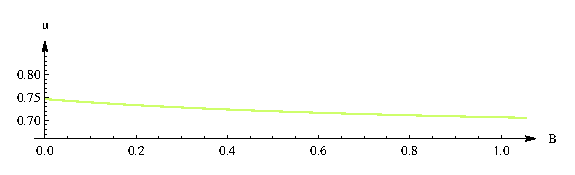
\includegraphics[width=0.9\textwidth]{C:/Users/BibiKiBa/Diss/Doktorarbeit/ModellEins/Abbildungen/uEL.eps}
\\
\hfill\footnotesize\sffamily{\textbf{Quelle:}}  eigene Darstellung
	\caption{Abhängigkeit des Anteils Humankapital $u$ im Produktionssektor einer relativ weniger weit entwickelten Volkswirtschaft von dem Offenheitsgrad $\bar{B}$}
	\label{fig:VeränderungHumankapitalOffenheitEL}
\end{figure}
\\
Das zusätzliche technologische Wissen durch den Import von relativ humankapitalreicheren Gütern führt zu einer Umverteilung des Humankapitalbestandes auf die beiden Sektoren Konsumgüterproduktion und Bildung. Mit steigender Offenheit, werden mehr Güter importiert, von denen technologisches Wissen absorbiert werden kann. Dementsprechend wird der Bildungssektor in einem weniger weit, jedoch geöffnetem Land produktiver und die Haushalte werden mehr Humankapital in den Bildungssektor investieren, als in den Konsumgutsektor. Dementsprechend sinkt mit steigender Offenheit der Parameter $u$, wie aus Abbildung \ref{fig:VeränderungHumankapitalOffenheitEL} entnommen werden kann.\\
Ein ähnlicher Zusammenhang wird in Abbildung \ref{fig:ChiEL} dargestellt. Je stärker sich ein Land öffnet, oder je eher es Freihandel zulässt, desto höher ist die Konsum-Kapitalquote, die den optimalen Wachstumspfad bedingt. 
%ABBILDUNG \\
\begin{figure}[htb] 
\vspace{0.23cm}
 \centering 
 \psfrag{B}{$\bar{B}$}
		\psfrag{Chi}{$\chi$}
		\psfrag{0.0}[c]{\footnotesize{0}}
		\psfrag{0.2}[c]{\footnotesize{0.2}}
		\psfrag{0.4}[c]{\footnotesize{0.4}}
		\psfrag{0.6}[c]{\footnotesize{0.6}}
		\psfrag{1.2}[c]{\footnotesize{1.2}}
		\psfrag{1.4}[c]{\footnotesize{1.4}}
		\psfrag{1.6}[c]{\footnotesize{1.6}}
		\psfrag{0.8}[c]{\footnotesize{0.8}}
		%\psfrag{0.80}[l]{\footnotesize{0.8}}
		%\psfrag{0.9}[]{\footnotesize{0.9}}
		\psfrag{1.0}[c]{~\footnotesize{1.0}}
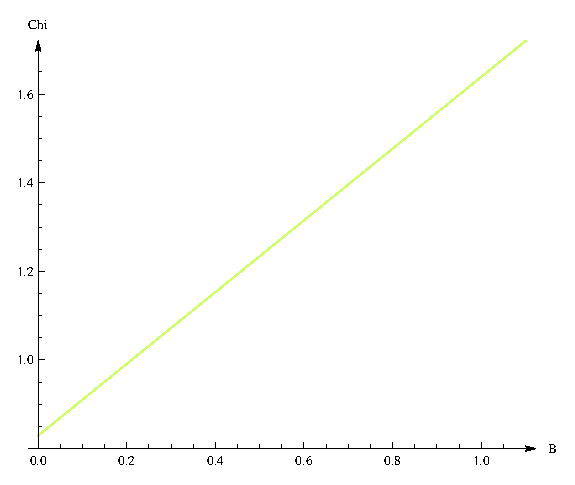
\includegraphics[width=0.54\textwidth]{C:/Users/BibiKiBa/Diss/Doktorarbeit/ModellEins/Abbildungen/ChiEL.eps}
\\
\hfill\footnotesize\sffamily{\textbf{Quelle:}}  eigene Darstellung
	\caption{Abhängigkeit der Kapital-Konsumquote $\chi$ einer relativ weniger weit entwickelten Volkswirtschaft von dem Offenheitsgrad $\bar{B}$}
	\label{fig:ChiEL}
\end{figure}
\\
Unter Berücksichtigung dieser berechneten optimalen Werte ergibt sich das gleichgewichtige Wirtschaftswachstum, das auch als Keynes-Ramsey-Regel bezeichnet wird. 
\begin{equation}
\boxed{\hat{c}^*=\frac{1}{\sigma}\left(\frac{1}{\alpha} B(1+\bar{B})-\rho\right)}
\end{equation}
Auch hier wird der positive Einfluss des Offenheitsparameters deutlich. Insgesamt wird die Wachstumsrate einer weniger weit entwickelten Volkswirtschaft durch Au{\ss}enhandel ansteigen, siehe Abbildung \ref{fig:cDachEL}.  
%ABBILDUNG 
\begin{figure}[htb] 
\vspace{0.23cm}
 \centering 
 \psfrag{B}{$\bar{B}$}
		\psfrag{cDach}{$\hat{c}$}
		\psfrag{0.0}[c]{\footnotesize{0}}
		\psfrag{0.2}[c]{\footnotesize{0.2}}
		\psfrag{0.4}[c]{\footnotesize{0.4}}
		\psfrag{0.6}[c]{\footnotesize{0.6}}
		\psfrag{0.9}[c]{\footnotesize{0.9}}
		\psfrag{0.7}[l]{\footnotesize{0.7}}
		\psfrag{0.75}[l]{\footnotesize{0.75}}
		\psfrag{0.8}[l]{\footnotesize{0.8}}
		%\psfrag{0.80}[l]{\footnotesize{0.8}}
		\psfrag{0.9}[l]{\footnotesize{0.9}}
		\psfrag{1.0}[l]{~\footnotesize{1}}
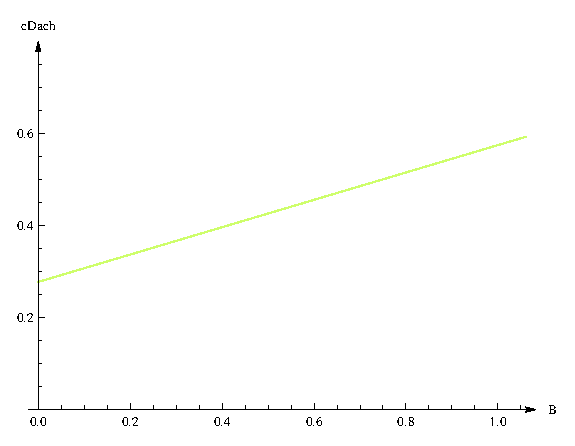
\includegraphics[width=0.54\textwidth]{C:/Users/BibiKiBa/Diss/Doktorarbeit/ModellEins/Abbildungen/cDachEL.eps}
\\
\hfill\footnotesize\sffamily{\textbf{Quelle:}}  eigene Darstellung
	\caption{Abhängigkeit der Wachstumsrate $\hat{c}$ einer relativ weniger weit entwickelten Volkswirtschaft von dem Offenheitsgrad $\bar{B}$}
	\label{fig:cDachEL}
\end{figure}

\FloatBarrier
\subsection{Handel in einem relativ weiter entwickelten Land}
Wird jetzt ein anderes Szenario betrachtet und von einem Land ausgegangen, dass relativ zum Weltmarkt weiter entwickelt ist, kann auch hier der Einfluss von Au{\ss}enhandel auf die intertemporale Konsumentscheidung gezeigt werden. Der Entwicklungsstand lässt sich aus der relativen Ausstattung des Sachkapitals zum Humankapital herleiten. Das Grenzprodukt im Bildungssektor eines weiter entwickelten Landes ist höher als das des relativ weniger weit entwickelten Weltmarktes. Somit gilt grundsätzlich, dass tendenziell mehr Humankapital akkumuliert wird und beide Produktionsfaktoren im Bildungssektor verwendet werden. In einem sehr weit entwickelten Land werden bei der Ausbildung von Schneidern nicht nur die Lehrkraft als Humankapital eingesetzt, sondern auch die Nähmaschinen als Sachkapital. Ebenfalls denkbar wäre eine Schulung über Medien wie Tablets, die mittels Videos die zu erlernenden Fähigkeiten verbreiten.\\ Ein relativ weiter entwickeltes Land verfügt demnach über relativ mehr Humankapital als Sachkapital, verglichen mit dem weniger weit entwickelten Land oder auch Weltmarkt. Es ergibt sich demnach die Bewegungsgleichung für das physische Kapital:
\begin{equation}
\dot{k}(t)=A(v(t)k(t))^\alpha(u(t)h(t))^{1-\alpha}-c(t)-c_{ex}(t)+p^*c_{im}(t)
\end{equation}
Das physische Kapital verändert sich über die Zeit, dahingehend, dass von dem produzierten Gütermengen gemä{\ss} $y=A(v(t)k(t))^\alpha(u(t)h(t))^{1-\alpha}$ und den bewerteten importierten Gütermengen $p^*c_{im}(t)$ die konsumierten Güter des Inlandes $c(t)$ sowie die exportierten Güter $c_{ex}(t)$ für das Ausland abgezogen werden. Die Kapitalakkumulation unterscheidet sich vom relativ weniger weit entwickelten Land nur durch den Faktor $v$, der den Anteil des Humankapitals bestimmt, der im Konsumgutsektor für die Produktion eingesetzt wird.\\   
Wie bereits angeführt, wird angenommen, dass in einem relativ weiter entwickelten Land für die Bildung neben Humankapital auch physisches Kapital eingesetzt wird.
\begin{equation}
\dot{h}(t)=B(1+\bar{B})((1-v(t))k(t))^{\eta}((1-u(t))h(t))^{1-\eta}
\end{equation}
Humankapital wird hier prinzipiell genauso akkumuliert, wie auf dem Weltmarkt, bzw. in der geschlossenen Referenzsituation, unter Berücksichtigung beider Kapitalarten. Demzufolge entwickelt sich das Humankapital über die Zeit, durch den Einsatz von Humankapital mit $((1-u(t))h(t))^{1-\eta}$ und von physischem Kapital mit $((1-v(t))k(t))^{\eta}$. Au{\ss}erdem beeinflussen auch hier die beiden Produktivitätsparameter $B$ und $\bar{B}$ den Bildungssektor.\footnote{Der Offenheitsparameter verhält sich ebenso wie in \eqref{Offenheit}.} Auch hier wird künftig wieder auf die Notation der Abhängigkeit der Variablen gegenüber der Zeit $t$ verzichtet.\\
Aus den Bewegungsgleichungen lassen sich die Wachstumsraten beider Kapitalarten herleiten: 
\begin{equation}
\hat{k}=Av^\alpha k^{\alpha-1}(uh)^{1-\alpha}-\frac{c}{k}-\frac{c_{ex}}{k}+p^*\frac{c_{im}}{k}\label{kHut}
\end{equation}
\begin{equation}
\hat{h}=B(1+\bar{B})\left[(1-v)\frac{k}{h}\right]^{\eta}(1-u)^{1-\eta}
\end{equation}
Die Relationen des physischen Kapitals zur Konsummenge lassen sich hier wieder verkürzt darstellen als $\chi=\frac{c}{k}$, $\chi_{ex}=\frac{c_{ex}}{k}$ sowie $\chi_{im}=\frac{c_{im}}{k}$. Eingesetzt in \eqref{kHut} ergibt sich zunächst:
\begin{equation}
\hat{k}=Av^\alpha u^{1-\alpha}\left(\frac{k}{h}\right)^{\alpha-1}-\chi-\chi_{ex}+p^*\chi_{im}
\end{equation}
Durch die Substitution von $x_1=\frac{vk}{uh}$ und $x_2=\frac{(1-v)k}{(1-u)h}$ lassen sich die Wachstumsraten wieder verkürzt darstellen.\\ 
\begin{equation}
\boxed{\hat{k}=Ax_1^\alpha \frac{uh}{k}-\chi-\chi_{ex}+p^*\chi_{im}}
\end{equation}
\begin{equation}
\boxed{\hat{h}=B(1+\bar{B})x_2^\eta(1-u)}
\end{equation}
Erneut wird das Maximierungsproblem mit der Hamiltonfunktion, dem Maximumprinzip, gelöst. Es soll der optimale Konsumpfad gefunden werden, der den Lebenszeitnutzen eines Individuums maximiert, der in einer relativ weiter entwickelten Volkswirtschaft lebt, die handelsoffen ist.
\begin{equation}
\begin{split}
\mathbb{H}=&~e^{-\rho t}\frac{(c^\beta c_{im}^{1-\beta})^{1-\sigma}}{1-\sigma}\\
&+\gamma_1(A(vk)^\alpha(uh)^{1-\alpha}-c-c_{ex}+p^*c_{im})\\
&+\gamma_2B(1+\bar{B})[(1-v)k]^{\eta}[(1-u)h]^{1-\eta}\\
\end{split}
\end{equation}
Beschrieben wird dieser Konsumpfad durch folgendes Gleichungssystem: 
\begin{align}
&\frac{\partial\mathbb{H}}{\partial c}\overset{!}{=}~0\label{eq:lfoc1IL}\\
&\frac{\partial\mathbb{H}}{\partial c_{im}}\overset{!}{=}~0\label{eq:lfoc1imIL}\\
&\frac{\partial\mathbb{H}}{\partial v}\overset{!}{=}~0\label{eq:lfoc2IL}\\
&\frac{\partial\mathbb{H}}{\partial k}\overset{!}{=}-\dot{\gamma_1}\label{eq:lfoc3IL}\\
&\frac{\partial\mathbb{H}}{\partial k}\overset{!}{=}-\dot{\gamma}_{1im}\label{eq:lfoc3imIL}\\
&\frac{\partial\mathbb{H}}{\partial u}\overset{!}{=}~0\label{eq:lfoc4IL}\\
&\frac{\partial\mathbb{H}}{\partial h}\overset{!}{=}-\dot{\gamma_2}\label{eq:lfoc5IL}
\end{align}
Die Bedingungen des relativ weiter entwickelten Landes ähneln den beiden zuvor beschriebenen Zuständen auf unterschiedliche Art und Weise. Die Ähnlichkeit zur Referenzsituation ist gegeben, da hier das Humankapital auf die gleiche Art akkumuliert wird. Dem relativ weniger weit entwickelten Land ähnelt der Wachstumspfad, da es sich bei beiden um offene Volkswirtschaften handelt und somit die Offenheitsparameter diesen beeinflussen. Die ausführliche Berechnung der Bedingungen erster Ordnung ist wieder in Appendix \ref{APPENDIXIL} zu finden. Zusammenfassend befindet sich eine relativ weiter entwickelte Volkswirtschaft dann im Gleichgewicht, wenn folgenden Restriktionen zutreffen.
\begin{align}
&\gamma_1=e^{-\rho t}\beta c^{\beta-1}c_{im}^{1-\beta}(c^\beta c_{im}^{1-\beta})^{-\sigma}\label{eq:foc1IL}\\
&\gamma_{1im}=-e^{-\rho t}(1-\beta) c^{\beta}c_{im}^{-\beta}(c^\beta c_{im}^{1-\beta})^{-\sigma}\label{eq:foc1imIL}\\
&\gamma_1A\alpha v^{\alpha-1}k^\alpha(uh)^{1-\alpha}=\gamma_2B(1+\bar{B})\eta(1-v)^{\eta-1}k^\eta[(1-u)h]^{1-\eta}\label{eq:foc2IL}\\
&\gamma_{1}A\alpha v^{\alpha} k^{\alpha -1} (u h)^{1- \alpha} + \gamma_{2}B(1+\bar{B})(1- v)^{\eta} k^{\eta -1} \eta \left [ (1-u)h \right ]^{1- \eta}= - \dot{\gamma}_{1}\label{eq:foc3IL}\\
&\gamma_{1 im}A\alpha v^{\alpha}k^{\alpha -1}(uh)^{1- \alpha}+ \gamma_{2}B(1+\bar{B}) [h(1-u)]^{1- \eta} \eta(1-v)^{\eta}k^{\eta -1}= - \dot{\gamma}_{1im}\label{eq:foc3imIL}\\
&\gamma_1A(1-\alpha)(vk)^{\alpha}u^{-\alpha}h^{1-\alpha}=\gamma_2B(1+\bar{B})(1-\eta)[(1-v)k]^\eta (1-u)^{-\eta} h^{1-\eta}\label{eq:foc4IL}\\
&\gamma_1A(1-\alpha)(vk)^\alpha u^{1-\alpha}h^{-\alpha}+\gamma_2 B(1+\bar{B})(1-\eta)[(1-v)k]^{\eta}(1-u)^{1-\eta}h^{-\eta}=-\dot{\gamma}_2\label{eq:foc5IL}
\end{align}
\vspace{-0.6cm}
\begin{equation}
\lim_{t \to \infty}e^{-\rho t}\gamma_1k=0;\qquad \lim_{t \to \infty}e^{-\rho t}\gamma_{1im}k=0; \qquad \lim_{t \to \infty}e^{-\rho t}\gamma_2h=0
\end{equation}
Auch hier wird in Gleichung \eqref{eq:foc1IL} zunächst der Schattenpreis einer zusätzlichen Einheit Kapital beschrieben. Dieser daraus resultierende zukünftige Lebenszeitgrenznutzen muss dem gegenwärtigen Nutzen entsprechen, der aus einer zusätzliche konsumierten Einheit resultiert. Der gleiche Zusammenhang, jedoch auf das importierte Gut $c_{im}$ bezogen beschreibt Gleichung \eqref{eq:foc1imIL}.\\
Bedingung \eqref{eq:foc2IL} und Gleichung \eqref{eq:foc4IL} gewährleisten, dass eine Volkswirtschaft erst dann im Gleichgewicht ist, wenn sich die mit dem jeweiligen Schattenpreis bewerteten Grenzprodukte entsprechen.\\
Die verbleibenden drei Bedingungen \eqref{eq:foc3IL}, \eqref{eq:foc3imIL} und \eqref{eq:foc5IL} beschreiben jeweils die Abschreibungsrate des Schattenpreises. Die durch Au{\ss}enhandel im relativ weiter entwickelten Land höher sind, als in der Referenzsituation ohne Handel. Der Nutzwert einer zusätzlichen Kapitaleinheit ist somit höher und muss damit auch über die Lebenszeit stärker abgeschrieben werden. 

\subsubsection*{Modelldynamik}
Aus den angeführten Bedingungen lassen sich die Keynes-Ramsey-Regeln, also die Konsumwachstumsraten für das heimisch produzierte und das importierte Konsumgut herleiten. 
\begin{equation}
\boxed{
\hat{c}=\frac{1}{(1-\beta+\sigma\beta)}\left(A\alpha x_1^{\alpha -1}-\rho+\hat{c}_{im}(1-\beta+\sigma\beta-\sigma)\right)}
\end{equation}
\begin{equation}
\boxed{
\hat{c}_{im}=\frac{1}{\beta-\sigma\beta+ \sigma}\left(A\alpha x_1^{\alpha -1}-\rho+\hat{c}(\beta - \sigma\beta)\right)}
\end{equation}
Beide Wachstumsraten bedingen sich gegenseitig, denn je nach Höhe der Konsum\-güter\-einfuhr kann weniger von den inländisch produzierten Gütern konsumiert werden und umgekehrt.\\
Ebenso wie in der Autarkiesituation entsprechen sich die Verhältnisse der Grenzproduktivitäten beider Sektoren.\footnote{Die Herleitung folgt aus den Gleichungen \eqref{eq:foc2IL} und \eqref{eq:foc3IL}, siehe dazu Appendix \ref{APPENDIXIL}.}
\begin{equation}
\boxed{\frac{1-\alpha}{\alpha}x_1=\frac{1-\eta}{\eta}x_2}
\end{equation}
In diesem Fall beeinflusst der Au{\ss}enhandel die Grenzproduktivitäten nicht. Die Grenzproduktivität einer marginalen Veränderung des Sach- oder Humankapitals im Konsumgutsektor sowie im Bildungssektor entsprechen sich, unabhängig von internationalen Einflüssen.\\
Dass die Wachstumsrate des Schattenpreises des physischen Kapitals dem Grenzprodukt des Kapitals entspricht, wird ist in der folgenden Gleichung formuliert. 
\begin{equation}\boxed{
B(1+\bar{B})(1-\eta)x_2^\eta=-\rho-\hat{c}(\beta-1-\sigma\beta)-\hat{c}_{im}(1-\beta+\sigma\beta-\sigma)-\alpha\hat{x}_1+\eta\hat{x}_2}
\end{equation}
Diese Schreibweise zeigt den Einfluss des Importgüterwachstums, sofern noch kein Au{\ss}enhandelsgleichgewicht angenommen wird, auf das Grenzprodukt des Kapitals im Konsumgutsektor. Das Grenzprodukt des Humankapitals im Bildungssektor ist aufgrund der Handelsbeziehungen, hier abgebildet durch den Offenheitsgrad $\bar{B}$, höher als in der Autarkiesituation. Beide Grenzprodukte und somit auch die Lebenszeitgrenznutzenwachstumsrate entsprechen sich auch in einer offenen Volkswirtschaft.
Der optimale Wachstumspfad eines offenen relativ weiter entwickelten Landes wird durch das folgende Gleichungssystem beschrieben. 
\begin{align}
&\hat{k}=Ax_1^\alpha \frac{uh}{k}-\chi-\chi_{ex}+p^*\chi_{im}\\
&\hat{h}=B(1+\bar{B})x_2^\eta(1-u)\\
& x_1(1-\alpha)/\alpha =x_2(1-\eta)/\eta\\
&\hat{c}=\frac{1}{(1-\beta+\sigma\beta)}\left(A\alpha x_1^{\alpha -1}-\rho+\hat{c}_{im}(1-\beta+\sigma\beta-\sigma)\right)\\
&\hat{c}_{im}=\frac{1}{\beta-\sigma\beta+ \sigma}\left(A\alpha x_1^{\alpha -1}-\rho+\hat{c}(\beta - \sigma\beta)\right)\\
&B(1+\bar{B})(1-\eta)x_2^\eta=-\rho-\hat{c}(\beta-1-\sigma\beta)-\hat{c}_{im}(1-\beta+\sigma\beta-\sigma)-\alpha\hat{x}_1+\eta\hat{x}_2
\end{align}
Für die Bestimmung des Gleichgewichts sind jedoch auch hier die einzelnen Werte zu berechnen. Für die exakte Berechnung aller weiteren Variablen werden die gleichgewichtigen Relationen $x_1$ und $x_2$ benötigt, dessen Wachstum konstant ist,  
\colorbox{lightgray}{$\hat{x}_1=\hat{x}_2=0$}. Aus dem Gleichungssystem ergibt sich: 
\begin{equation}
x_2^*=\left(\frac{\rho+\sigma\hat{c}}{B(1+\bar{B})(1-\eta)}\right)^{1/\eta}
\end{equation}
\begin{equation}
x_1^* =\frac{\alpha(1-\eta)}{\eta(1-\alpha)}\left(\frac{\rho+\sigma\hat{c}}{B(1+\bar{B})(1-\eta)}\right)^{1/\eta}
\end{equation}
Wird davon ausgegangen, dass sich die Volkswirtschaft auch im Au{\ss}enhandelsgleichgewicht befindet, dann entsprechen sich beide Konsumgüterwachstumsraten \colorbox{lightgray}{$\hat{c}=\hat{c}_{im}$}. 
\begin{equation}
\hat{c}=\frac{1}{\sigma}(A\alpha x_1^{\alpha-1}-\rho)
\end{equation}
Daraus ergibt sich das gleichgewichtige Konsumwachstum einer geöffneten Volkswirtschaft eines relativ weiter entwickelten Landes, das sich hinsichtlich des Offenheitsparameter $\bar{B}$ von der hiesigen im Autarkiezustand unterscheidet.
\begin{equation}
\boxed{\hat{c}^*=\frac{1}{\sigma}\left(\left[A^\eta\alpha^{\alpha\eta}(1-\eta)^{(1-\eta)(1-\alpha)}(\eta(1-\alpha))^{\eta(1-\alpha)}(B(1+\bar{B}))^{1-\alpha}\right]^\frac{1}{1+\eta-\alpha}-\rho\right)}
\end{equation}
Je offener eine Volkswirtschaft ist und desto mehr technisches Wissen durch den Import von Gütern absorbiert werden kann, desto höher ist die Wachstumsrate.\footnote{In diesem Abschnitt wird das Grenzprodukt der Übersichtlichkeit halber verkürzt durch $\bar{M}=\left[A^\eta\alpha^{\alpha\eta}(1-\eta)^{(1-\eta)(1-\alpha)}(\eta(1-\alpha))^{\eta(1-\alpha)}(B(1+\bar{B}))^{1-\alpha}\right]^\frac{1}{1+\eta-\alpha}$} Dieser Zusammenhang ist auch der folgenden Abbildung \ref{fig:cDachIL} zu entnehmen. 
%ABBILDUNG 
\begin{figure}[htb] 
\vspace{0.23cm}
 \centering 
 \psfrag{B}{$\bar{B}$}
		\psfrag{cDAch}{$\hat{c}$}
		\psfrag{0.0}[c]{\footnotesize{0}}
		\psfrag{0.2}[c]{\footnotesize{0.2}}
		\psfrag{0.4}[c]{\footnotesize{0.4}}
		\psfrag{0.6}[c]{\footnotesize{0.6}}
		\psfrag{0.05}[c]{\footnotesize{0.05}}
		\psfrag{0.10}[c]{\footnotesize{0.10}}
		\psfrag{0.15}[c]{\footnotesize{0.15}}
		\psfrag{0.8}[l]{\footnotesize{0.8}}
		%\psfrag{0.80}[l]{\footnotesize{0.8}}
		\psfrag{0.9}[l]{\footnotesize{0.9}}
		\psfrag{1.0}[l]{~\footnotesize{1}}
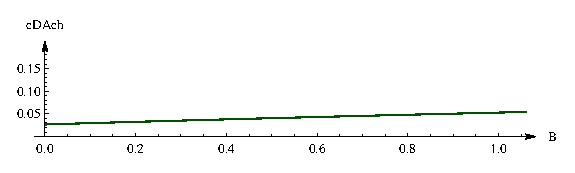
\includegraphics[width=0.9\textwidth]{C:/Users/BibiKiBa/Diss/Doktorarbeit/ModellEins/Abbildungen/cDachIL.eps}
\\
\hfill\footnotesize\sffamily{\textbf{Quelle:}}  eigene Darstellung
	\caption{Abhängigkeit der Wachstumsrate $\hat{c}$ einer relativ weiter entwickelten Volkswirtschaft von dem Offenheitsgrad $\bar{B}$}
	\label{fig:cDachIL}
\end{figure}
\\
Auch hier wird die gleichgewichtige optimale Aufteilung des Kapitals auf die beiden Sektoren Bildung und Konsumgüterproduktion ermittelt, dadurch, dass die Rate des Humankapitalwachstums der des Konsumgüterwachstums entspricht, \colorbox{lightgray}{$\hat{c}=\hat{h}$}.
\begin{equation}
\boxed{u^*=\frac{\sigma \bar{M}-(1-\eta)(\bar{M}-\rho)}{\sigma \bar{M}}}
\end{equation}
Diese Gleichung zeigt, dass Au{\ss}enhandel in einem relativ weiter entwickelten Land über das Grenzprodukt $\bar{M}$ Einfluss auf die Entscheidung hat, weniger Humankapital in den Konsumgütersektor zu investieren. Je mehr Technologietransfer durch steigende Offenheit $\bar{B}$ stattfindet, desto weniger Humankapital wird in den Produktionsprozess eingehen und dafür den Bildungssektor unterstützen, aufgrund eines Anstiegs von $(1-u)$. Dieser Zusammenhang ist in Abbildung \ref{fig:VeränderungHumankapitalOffenheit} dargestellt.  \\%ABBILDUNG
\begin{figure}[htb!] 
\vspace{0.13cm}
 \centering 
 \psfrag{B}{$\bar{B}$}
		\psfrag{u}{  $u$}
		\psfrag{0.0}[l]{\footnotesize{0}}
		\psfrag{0.2}[l]{\footnotesize{0.2}}
		\psfrag{0.4}[l]{\footnotesize{0.4}}
		\psfrag{0.6}[l]{\footnotesize{0.6}}
		\psfrag{0.70}[l]{\footnotesize{0.7}}
		\psfrag{0.75}[l]{\footnotesize{0.75}}
		\psfrag{0.8}[l]{\footnotesize{0.8}}
		\psfrag{0.80}[l]{\footnotesize{0.80}}
		\psfrag{0.85}[l]{\footnotesize{0.85}}
		\psfrag{0.90}[l]{\footnotesize{0.90}}
		\psfrag{1.0}[l]{~\footnotesize{1}}
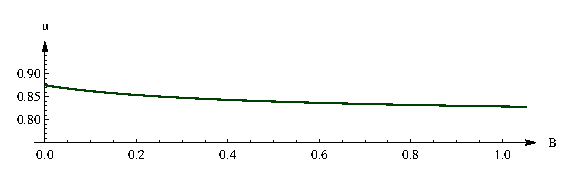
\includegraphics[width=0.9\textwidth]{C:/Users/BibiKiBa/Diss/Doktorarbeit/ModellEins/Abbildungen/uIL.eps}
\\
\hfill\footnotesize\sffamily{\textbf{Quelle:}}  eigene Darstellung
	\caption{Abhängigkeit des Anteils Humankapital $u$ im Produktionssektor einer relativ weiter entwickelten Volkswirtschaft von dem Offenheitsgrad $\bar{B}$}
	\label{fig:VeränderungHumankapitalOffenheit}
\end{figure}
\\
Nicht nur durch die Umverteilung des Humankapitals führt Freihandel zum Anstieg qualifizierter Arbeitskräfte, sondern es wird durch die Verteilung des Sachkapitals $v$ auf die beiden Sektoren auch das Bildungssystem gefördert. 
\begin{equation}
\boxed{
v^*=\frac{\alpha  (1-\eta ) \left(\frac{\bar{M}}{B (1+\bar{B}) (1-\eta )}\right)^{1/\eta } (\bar{M} \sigma -(1-\eta ) (\bar{M}-\rho ))}{(1-\alpha ) \eta  \bar{M} \sigma  \left(\frac{\alpha  (1-\eta ) \left(\frac{\bar{M}}{B (1+\bar{B}) (1-\eta )}\right)^{1/\eta } (\bar{M} \sigma -(1-\eta ) (\bar{M}-\rho ))}{(1-\alpha ) \eta  \bar{M} \sigma }+\left(\frac{\bar{M}}{B (1+\bar{B}) (1-\eta )}\right)^{1/\eta } \left(1-\frac{\bar{M} \sigma -(1-\eta ) (\bar{M}-\rho )}{\bar{M} \sigma }\right)\right)}}
\end{equation}
Ebenso verhält es sich mit der Aufteilung des Sachkapitals. Auch hier wirkt die Offenheit im Grenzprodukt als primärer Einflussfaktor zugunsten des Bildungssektors.\\ Abbildung \ref{fig:VeränderungSachkapitalOffenheit} stellt die negative Abhängigkeit des auf den Konsumgutsektor entfallenden Anteil des Sachkapitals $v$ zu der Offenheit dar. 
%ABBILDUNG
\begin{figure}[htb] 
\vspace{0.13cm}
 \centering 
 \psfrag{B}{$\bar{B}$}
		\psfrag{v}{  $v$}
		\psfrag{-}{  $_-$}
		\psfrag{1}{\, $_1$}
		\psfrag{0.0}[l]{\footnotesize{0}}
		\psfrag{0.2}[l]{\footnotesize{0.2}}
		\psfrag{0.4}[l]{\footnotesize{0.4}}
		\psfrag{0.6}[l]{\footnotesize{0.6}}
		\psfrag{0.70}[l]{\footnotesize{0.70}}
		\psfrag{0.75}[l]{\footnotesize{0.75}}
		\psfrag{0.8}[l]{\footnotesize{0.8}}
		\psfrag{0.80}[l]{\footnotesize{0.80}}
		\psfrag{1.0}[l]{~\footnotesize{1}}
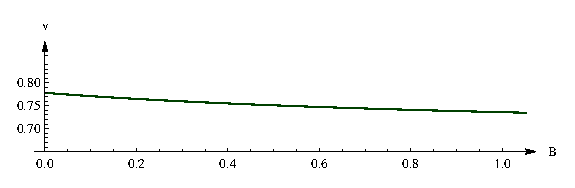
\includegraphics[width=0.9\textwidth]{C:/Users/BibiKiBa/Diss/Doktorarbeit/ModellEins/Abbildungen/vIL.eps}
\\
\hfill\footnotesize\sffamily{\textbf{Quelle:}}  eigene Darstellung
	\caption{Abhängigkeit des Anteils Sachkapital $v$ im Produktionssektor einer relativ weiter entwickelten Volkswirtschaft von dem Offenheitsgrad $\bar{B}$}
	\label{fig:VeränderungSachkapitalOffenheit}
\end{figure}
\\
Au{\ss}erdem ist es notwendig, dass die Kapital-Konsumquote $\chi$ im Gleichgewicht konstant ist. Dies gilt immer dann, wenn \colorbox{lightgray}{$\hat{c}=\hat{k}$} im Gleichgewicht gilt und ist ebenfalls abhängig vom Diffusionsparameter $\bar{B}$, siehe Abbildung \ref{fig:ChiIL}.
\begin{equation}
\boxed{\chi^*=\frac{1}{\sigma}\left(\frac{A\alpha \sigma[-\eta\rho+\bar{M}(\eta+\sigma-1)+\rho] \left(\frac{\alpha  (\eta -1) \left(\frac{\bar{M}}{B (1+\bar{B})(1-\eta) }\right)^{1/\eta }}{(\alpha -1) \eta }\right)^{\alpha -1}}{\rho  (\alpha -\eta )+\bar{M} (\alpha  (\sigma -1)+\eta )}-\bar{M}+\rho\right)}
\end{equation}
%ABBILDUNG 
\begin{figure}[h!] 
\vspace{0.23cm}
 \centering 
 \psfrag{B}{$\bar{B}$}
	\psfrag{Chi}{$\chi$}
		\psfrag{0.0}[c]{\footnotesize{0}}
		\psfrag{0.2}[c]{\footnotesize{0.2}}
		\psfrag{0.4}[l]{\footnotesize{0.4}}
		\psfrag{0.6}[l]{\footnotesize{0.6}}
		\psfrag{0.3}[l]{\footnotesize{0.3}}
		\psfrag{0.10}[c]{\footnotesize{0.10}}
		\psfrag{0.5}[l]{\footnotesize{0.5}}
		\psfrag{0.8}[c]{\footnotesize{0.8}}
		%\psfrag{0.80}[l]{\footnotesize{0.8}}
		\psfrag{0.9}[c]{\footnotesize{0.9}}
		\psfrag{1.0}[c]{~\footnotesize{1}}
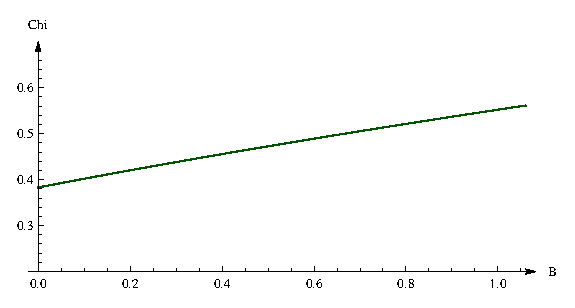
\includegraphics[width=0.9\textwidth]{C:/Users/BibiKiBa/Diss/Doktorarbeit/ModellEins/Abbildungen/ChiIL.eps}
\\
\hfill\footnotesize\sffamily{\textbf{Quelle:}}  eigene Darstellung
	\caption{Abhängigkeit der Kapital-Konsumquote $\chi$ einer relativ weiter entwickelten Volkswirtschaft von dem Offenheitsgrad $\bar{B}$}
	\label{fig:ChiIL}
\end{figure}

\subsection{Handelspolitik}
Bisher wurde nicht immer von der Offenheit eines Landes gesprochen ohne dabei auch die wohlfahrtsmindernde Wirkung protektionistischer Ma{\ss}nahmen zu berücksichtigen. Eingangs bei der Betrachtung des Offenheitsparameter $\bar{B}$ wurde impliziert, dass dieser geringer ist, wenn das Handelsvolumen kleiner ist. Dieses kleinere Handelsvolumen kann aus der aktiven Einschränkung des Handels durch Zölle, Kontingente, Subventionen oder auch nicht- tarifären Handelshemmnissen wie Richtlinien resultieren. Bei der folgenden Zusammenfassung des Einflusses von Au{\ss}enhandel auf den Entwicklungsprozess, kann somit zugleich von einer gegensätzlichen Wirkung von Handelshemmnissen ausgegangen werden. 
%\textcolor[rgb]{1,0,0}{(so drin lassen??? kommt in Kapitel Papier 1 nochmal handelshemmnis? ist diese Exportförderung ein Hemmnis???) }

\section{Zwischenfazit}
In diesem Kapitel wurde der Einfluss von Au{\ss}enhandel auf die Humankapitalakkumulation bei unterschiedlichen Entwicklungsständen untersucht. Verdeutlicht werden die Ergebnisse anhand eines Vergleichs beider Szenarien mit der Referenzsituation Autarkie. Durch den Anteil des Sachkapitals der in der Güterproduktion aufgewendet wird $v$, können auch indirekt Aussagen über den Bildungssektor getroffen werden, da sich der Anteil des physischen Kapitals im Bildungssektor aus $(1-v)$ ergibt. Der Vergleich der verschiedenen Entwicklungsstadien ist in Abbildung \ref{fig:VergleichV} dargestellt. In einem relativ \textcolor[rgb]{0,0.58,0}{weiter entwickelten Land} sinkt $v$ mit zunehmender Offenheit. Aus der Perspektive des Bildungssektors stellt sich dieser mit der Zunahme der Offenheit besser, als wenn ein Land geschlossen ist, da nun mehr Sachkapital im Bildungssektor eingesetzt wird.\\  %ABBILDUNG
\begin{figure}[htb] 
\vspace{0.13cm}
 \centering 
 \psfrag{B}{$\bar{B}$}
		\psfrag{v}{  $v$}
		\psfrag{0.0}[l]{\footnotesize{0}}
		\psfrag{0.2}[l]{\footnotesize{0.2}}
		\psfrag{0.4}[l]{\footnotesize{0.4}}
		\psfrag{0.6}[l]{\footnotesize{0.6}}
		\psfrag{0.7}[l]{\footnotesize{0.7}}
		\psfrag{0.75}[l]{\footnotesize{0.75}}
		\psfrag{0.8}[l]{\footnotesize{0.8}}
		%\psfrag{0.80}[l]{\footnotesize{0.8}}
		\psfrag{0.9}[l]{\footnotesize{0.9}}
		\psfrag{1.0}[l]{~\footnotesize{1}}
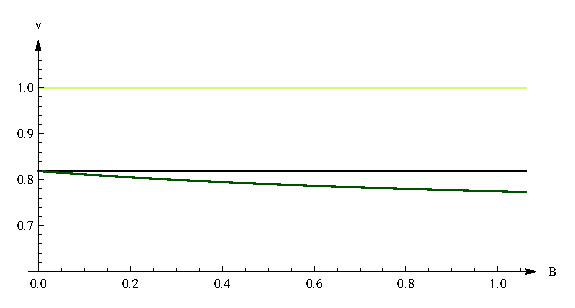
\includegraphics[width=0.9\textwidth]{C:/Users/BibiKiBa/Diss/Doktorarbeit/ModellEins/Abbildungen/VergleichV.eps}
\\
\hfill\footnotesize\sffamily{\textbf{Quelle:}}  eigene Darstellung
	\caption{Veränderung des Anteils Sachkapital $v$ im Produktionssektor unterschiedlicher Entwicklungsstadien abhängig von dem Offenheitsgrad $\bar{B}$}
	\label{fig:VergleichV}
\end{figure}
\\
Das Niveau der Entscheidungsvariablen $v$ der Haushalte aus \textcolor[rgb]{0.74,0.97,0.22}{weniger weit entwickelten Ländern} ist deutlich höher und konstant, da $v=1$. Somit wird das gesamte physische Kapital in die Güterproduktion eingehen. Durch den Verzicht des Einsatzes von physischem Kapital in den Bildungssektor, wird das Sachkapital komplett für die Produktion von Gütern verwendet und führt dazu, dass im Konsumgutsektor insgesamt weniger Humankapital eingesetzt werden muss. Dadurch wird der Haushalt deutlich mehr Humankapital in Bildungssektor investieren. Dieser Zusammenhang kann der Abbildung \ref{fig:VergleichU} entnommen werden. %\\ABBILDUNG
\begin{figure}[htb] 
\vspace{0.13cm}
 \centering 
 \psfrag{B}{$\bar{B}$}
		\psfrag{u}{  $u$}
		\psfrag{0.0}[c]{\footnotesize{0}}
		\psfrag{0.2}[c]{\footnotesize{0.2}}
		\psfrag{0.4}[c]{\footnotesize{0.4}}
		\psfrag{0.6}[c]{\footnotesize{0.6}}
		\psfrag{0.9}[c]{\footnotesize{0.9}}
		\psfrag{0.7}[c]{\footnotesize{0.7}}
		\psfrag{0.75}[l]{\footnotesize{0.75}}
		\psfrag{0.8}[c]{\footnotesize{0.8}}
		%\psfrag{0.80}[l]{\footnotesize{0.8}}
		\psfrag{0.9}[c]{\footnotesize{0.9}}
		\psfrag{1.0}[c]{~\footnotesize{1}}
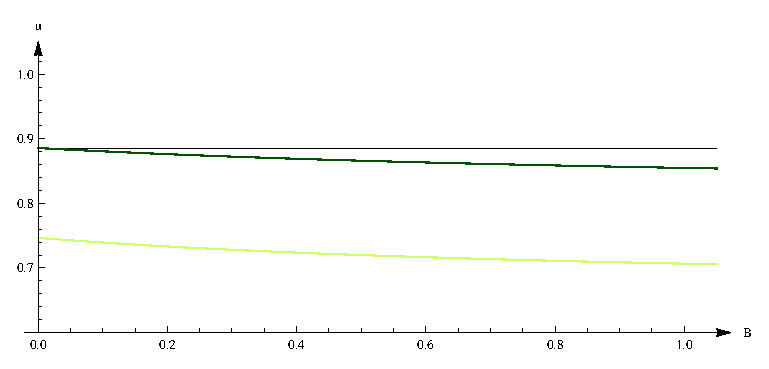
\includegraphics[width=0.9\textwidth]{C:/Users/BibiKiBa/Diss/Doktorarbeit/ModellEins/Abbildungen/VergleichU.eps}
\\
\hfill\footnotesize\sffamily{\textbf{Quelle:}}  eigene Darstellung
	\caption{Veränderung des Anteils Humankapital $u$ im Produktionssektor  unterschiedlicher Entwicklungsstadien abhängig von dem Offenheitsgrad $\bar{B}$}
	\label{fig:VergleichU}
\end{figure}
\\
Unabhängig von dem Entwicklungsstand kommt es immer zu einer Aufteilung des Humankapitals auf beide Sektoren. Durch Au{\ss}enhandel sinkt der Anteil des Humankapitals $u$, der in den Konsumgutsektor eingeht, demzufolge steigt der Anteil im Bildungssektor $(1-u)$ an. Jedoch gibt es auch hier Niveauunterschiede. In dem hier angeführten Beispiel werden die Haushalte eines \textcolor[rgb]{0.74,0.97,0.22}{weniger weit entwickelten Landes} ca. 25\% des Humankapitals von den Haushalten in den Bildungssektor einsetzen, dieser Anteil nimmt mit der Öffnung des Landes zu.\footnote{Da die relativ weniger weit entwickelten Länder nur Humankapital in den Bildungssektor investieren, kann das Sachkapital vollständig für die Konsumgüterproduktion verwendet werden. Demzufolge wird verhältnismä{\ss}ig weniger Humankapital (75\%) für die Produktion verwendet als in einem relativ weiter entwickelten Land (90\%). Der verbleibende höhere Anteil Humankapital kann nun zusätzlich in den Bildungssektor investiert werden. Demzufolge resultiert der angesprochene Niveauunterschied.} Haushalte in \textcolor[rgb]{0,0.58,0}{relativ weiter entwickelten Volkswirtschaften} werden auch weniger Humankapital in die Güterproduktion investiert, dafür aber immer mehr in den Bildungssektor je stärker sich das Land öffnet. Im Vergleich zur \textbf{Autarkiesituation} verbessert sich in beiden Situationen die Humankapitalakkumulation durch Freihandel. \\
Demzufolge entscheiden sich die Haushalte in geöffneten Volkswirtschaften zu Gunsten der eigenen Weiterbildung und gewichten somit das hinzugekommene technische Wissen stärker  als in einer geschlossenen Volkswirtschaft. Freihandel kann ein Ansatz sein, die Anreize der Bevölkerung zu erhöhen sich weiterzubilden, unabhängig vom Entwicklungsstand. \\
Die Öffnung eines Landes verstärkt den Wissenstransfer und die damit einhergehende Technologiediffusion. Das Modell zeigt, dass der Humankapitalbestand in relativ weniger weit entwickelten Volkswirtschaften durch Au{\ss}enhandel ansteigt und dadurch die Lücke zur übrigen Welt geschlossen werden kann. Denn der Technologietransfer wird verstärkt durch den Handel mit humankapitalreichen Gütern, die in das weniger weit entwickelte Land importiert werden. Dadurch steigt die Wachstumsrate dieses Landes an und konvergiert zum Weltmarktgleichgewicht. Diese Wirkung auf das Wirtschaftswachstum zeigt folgend die Abbildung \ref{fig:cDachVergleich}.  
%ABBILDUNG 
\begin{figure}[htb] 
\vspace{0.23cm}
 \centering 
 \psfrag{B}{$\bar{B}$}
		\psfrag{cDach}{$\hat{c}$}
		\psfrag{0.0}[c]{\footnotesize{0}}
		\psfrag{0.2}[c]{\footnotesize{0.2}}
		\psfrag{0.4}[c]{\footnotesize{0.4}}
		\psfrag{0.6}[c]{\footnotesize{0.6}}
		\psfrag{0.5}[c]{\footnotesize{0.5}}
		\psfrag{0.3}[c]{\footnotesize{0.3}}
		\psfrag{0.1}[c]{\footnotesize{0.1}}
		\psfrag{0.8}[c]{\footnotesize{0.8}}
		%\psfrag{0.80}[l]{\footnotesize{0.8}}
		\psfrag{0.9}[c]{\footnotesize{0.9}}
		\psfrag{1.0}[c]{~\footnotesize{1}}
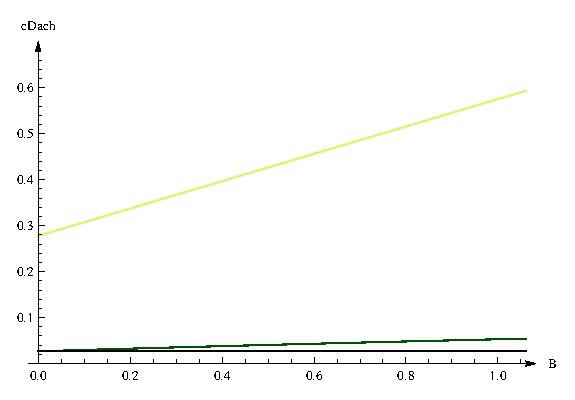
\includegraphics[width=0.7\textwidth]{C:/Users/BibiKiBa/Diss/Doktorarbeit/ModellEins/Abbildungen/cDachVergleich.eps}
\\
\hfill\footnotesize\sffamily{\textbf{Quelle:}}  eigene Darstellung
	\caption{Vergleich der Wachstumsraten $\hat{c}$ unterschiedlicher Entwicklungsstadien abhängig von dem Offenheitsgrad $\bar{B}$}
	\label{fig:cDachVergleich}
\end{figure}
\\
Die Referenzsituation einer \textbf{geschlossenen Volkswirtschaft} zeigt keine Abhängigkeit des Wirtschaftswachstums gegenüber der Offenheit. Die Produktionsstrukturen eines \textcolor[rgb]{0,0.58,0}{relativ weiter entwickelten Landes} sind denen der hier aufgeführten Autarkiesituation sehr ähnlich, da bei beiden $v>0$ gilt. Demzufolge ist das Wirtschaftswachstum beider Situationen einer geschlossenen Volkswirtschaft mit $\bar{B}=0$ noch gleich. Das offene relativ weiter entwickelte Land verzeichnet jedoch mit zunehmender Offenheit einen geringen Anstieg der Wachstumsrate.\\
Das \textcolor[rgb]{0.74,0.97,0.22}{weniger weit entwickelte Land} startet von einem deutlich höheren Wert der Wachstumsrate $\hat{c}$ bei $\bar{B}=0$ und verzeichnet noch eine stärkere Zunahme der Wachstumsrate mit steigender Offenheit $\bar{B}$. Dieser recht steile Anstieg spiegelt den Aufholprozess weniger weit entwickelter Länder wieder. Die Veränderung des Grenzproduktes ist in weniger weit entwickelten Volkswirtschaften noch höher und führt somit auch zu einer höheren Wachstumsrate. Hinzu kommt, dass der Wissenstransfer für ein weniger weit entwickeltes Land deutlich höher ist und Wissen aufholen kann, als ein relativ weiter entwickeltes Land.\\
Im Ergebnis zeigt diese Abbildung, dass unabhängig vom Entwicklungsstand und den damit einhergehenden Bildungssystemen Freihandel zu einer höheren Wachstumsrate führt. \\
In dem folgenden Kapitel wird ein Modell vorgestellt, dass den technischen Fortschritt beschreibt und das hier akkumulierte Humankapital zu Imitationen bzw. Innovationen umwandelt. Die Anwendung, Implementierung und Entwicklung neuer Technologien benötigt qualifizierte Arbeit. So bestätigen auch \citet{Nelson.1966} die Bedeutung des Humankapital für den technischen Fortschritt einer Volkswirtschaft. Ein hoher Bildungsstand beschleunigt den Prozess der technischen Diffusion und, dass demzufolge eher Innovationen entwickelt werden. Daraus l{\"a}sst sich f{\"u}r diese Arbeit der Rückschluss ziehen, dass hohe Qualifikationen der Unternehmer f{\"u}r die Entwicklung von Innovationen notwendig sind und sich daraufhin f{\"u}r eine passende Strategie entschieden wird. Das folgende Modell wird daher die Bedeutung von F{\"a}higkeiten und Humankapital f{\"u}r die passende Entscheidung bezüglich einer Unternehmensstrategie und auch f{\"u}r den technischen Fortschritt betonen.